\documentclass[11pt,ngerman]{scrartcl}

% standard packages
\usepackage[utf8]{inputenc}  % input in UTF-8
\usepackage[T1]{fontenc}  % output in T1 fonts (westeuropäische Codierung)
\usepackage{lmodern}  % latin modern fonts
\usepackage[ngerman]{babel}  % deutsches Sprachpaket, neue Rechtschreibung

% Seitensetup
\usepackage{scrlayer-scrpage}  % Seitenformatierung durch KOMA-interne Optionen
\usepackage[top=4cm, bottom=4cm]{geometry}  % Seitengeometrie (kann durch KOMA ersetzt werden, hab ich aber nicht geschafft)
\usepackage[hypcap=false]{caption, subcaption}  % caption editing - hypcap warning with hyperref
\usepackage{array}  % table editing

% additional packages
\usepackage{amsmath, amssymb, amstext}  % math packages (American Math Society)
\usepackage{bm}
\usepackage{icomma}  % Kommata in Dezimalzahlen verursachen keinen Abstand mehr
\usepackage{graphicx}  % Bilder einfügen
\usepackage{float} %Bilder placement
\usepackage{pdfpages}  % PDF als vollständige Seiten einfügen
\usepackage{lastpage}  % referenziert die letzte Seite
\usepackage[separate-uncertainty=true]{siunitx}  % bessere Darstellung von Einheiten
\usepackage{makecell} %Dicke Tabellenstriche
\usepackage{longtable}
\usepackage{booktabs}
%\usepackage{datatool}
\usepackage[hidelinks]{hyperref}  % hyperref verlinkt Referenzen - hidelinks entfernt borders um links

% package setups
% Kopf- und Fußzeile durch KOMA
\pagestyle{scrheadings}  % KOMA darf entscheiden
\clearpairofpagestyles  % reset
\setkomafont{pageheadfoot}{\normalfont}  % Standardschrift in Kopf- und Fußzeile
\captionsetup{format=plain, font=small, labelfont=bf} %Better caption, Abbildung ist FETT
%\setlength{\headheight}{27.2pt}  % benötigte Höhe Kopfzeile (warning von scrlayer-scrpage, wird aber automatisch so gerendert, falls diese Option weggelassen wird)
\ihead{Spektralphotometer}  % Kopf links %Todo Titel ändern
\chead{\textsc{Philipp} Maximilian \\ \textsc{Stark} Matthias}  % Kopf Mitte %Todo Name ändern
\ohead{08 Oktober 2021}  % Kopf rechts %Todo Datum ändern
\cfoot{\pagemark \, / \pageref{LastPage}}  % Fuß Mitte

% Table of Contents
\DeclareTOCStyleEntry{dottedtocline}{section}  % KOMA intern - Inhaltsverzeichnis mit Punkten (nur sections)

%Overbar setup
\newcommand{\overbar}[1]{\mkern 1.5mu\overline{\mkern-1.5mu#1\mkern-1.5mu}\mkern 1.5mu}
% SI
\sisetup{locale = DE}  % deutschsprachige SI-Konvention
\sisetup{quotient-mode = fraction}
\sisetup{per-mode = fraction}
\DeclareSIUnit\px{px}
\DeclareSIUnit\strich{|||}

% citation
\usepackage{csquotes}
\usepackage[backend=biber]{biblatex}
\addbibresource{quincke-kundt.bib} %Todo .bib befüllen zb.: mit JabRef (Empfehlung der Redaktion)

%Eigene Commands
\newcommand{\der}[2]{\frac{\mathrm{d}#1}{\mathrm{d}#2}}
\newcommand{\pder}[2]{\frac{\partial #1}{\partial #2}}

\begin{document}
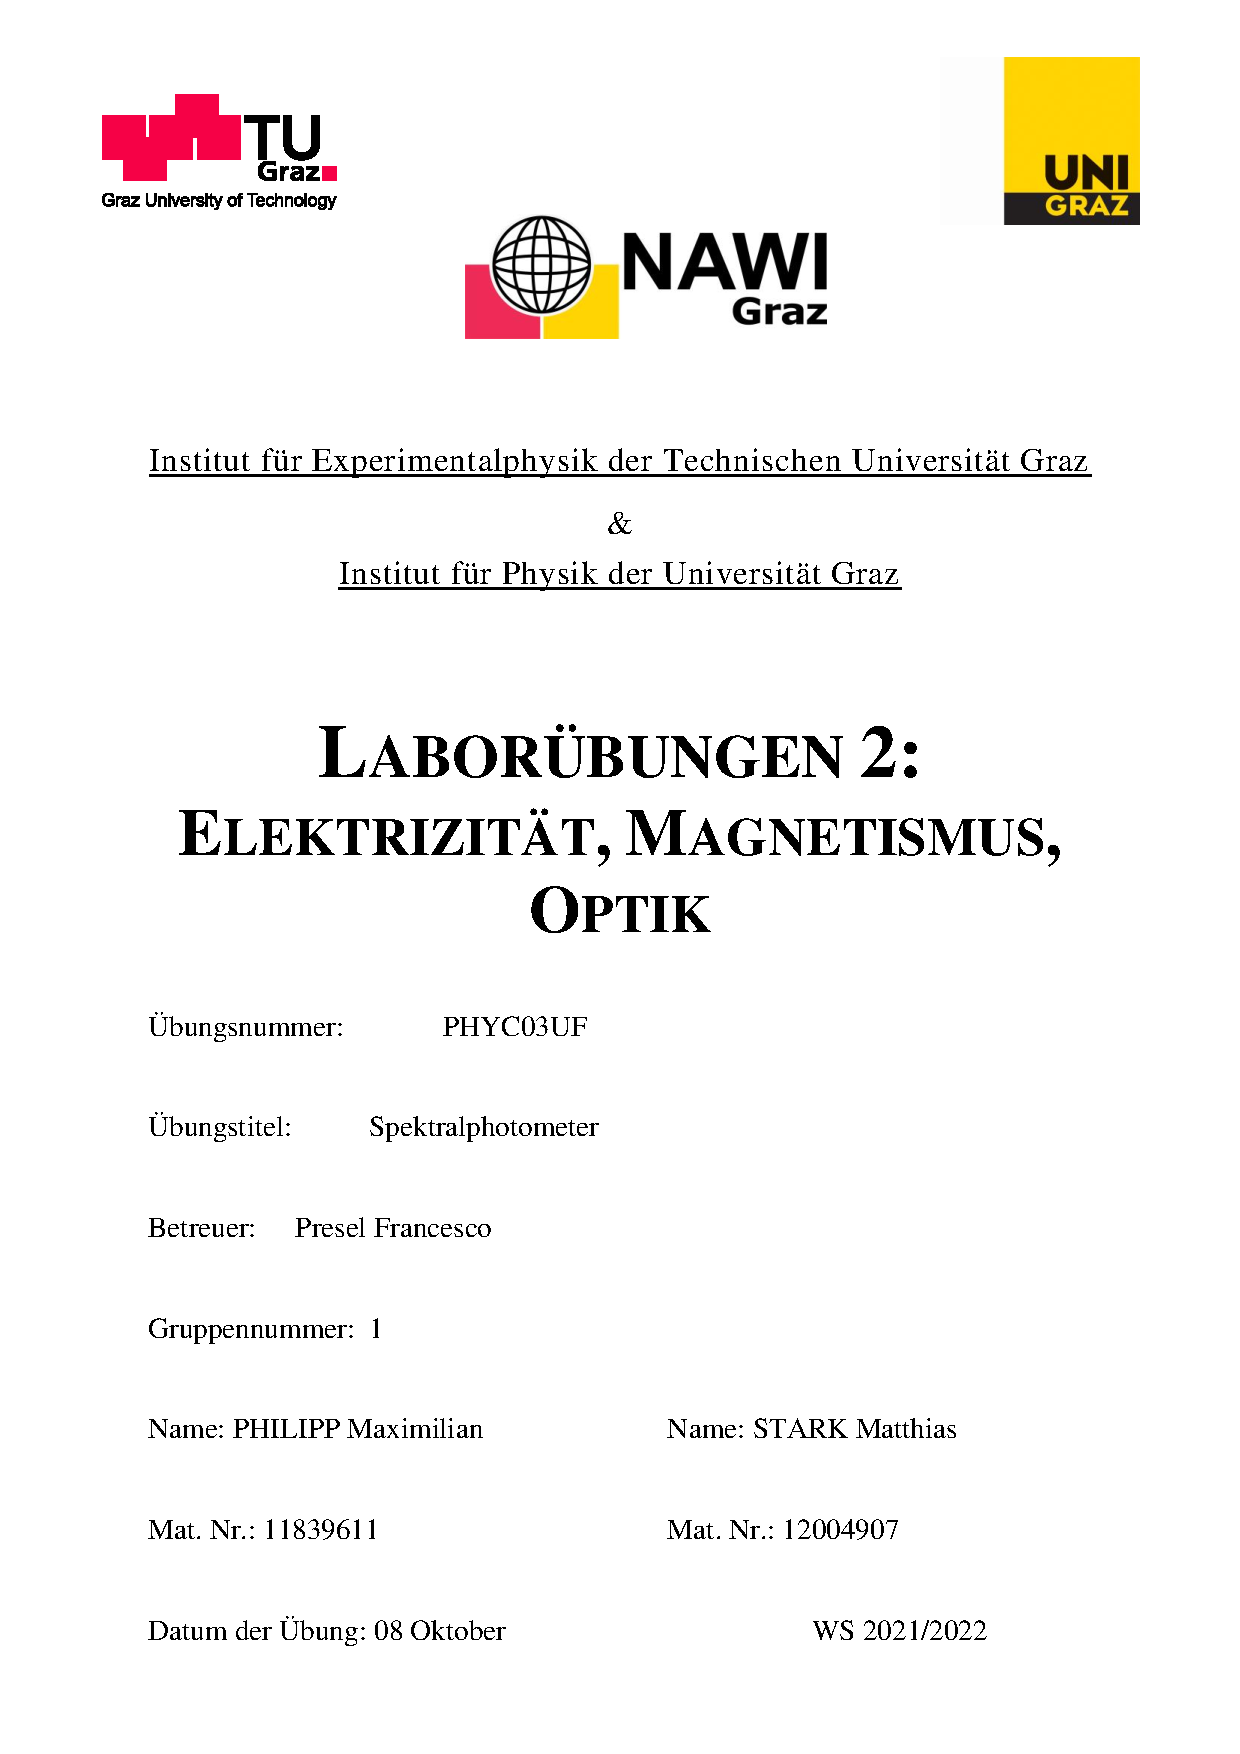
\includepdf{Deckblatt_Stark.pdf}
\tableofcontents
\newpage

\section{Aufgabenstellung\label{Auf0}}

\noindent Zunächst muss mit dem Spektralphotometer die optische Transmission
gemessen und diese gemeinsam mit der Extinktion als Funktion der
Lichtwellenlänge dargestellt werden. Dabei soll Additivität der Extinktion
gezeigt werden.

\vspace{2mm}

\noindent Weiters soll die Stoffmengenkonzentration einer Methylenblaulösung
bestimmt werden.

\vspace{2mm}

\noindent Zusätzlich soll die Dicke einer Glasplatte durch Auswertung der
Interferenzmaxima im Transmissionsspektrum ermittelt werden. \cite{spektovorlage}


\section{Grundlagen}

\noindent Um den Versuch durchführen zu könne, müssen die Begriffe der
Transmission, Extinktion und Absorbtionsquerschnitt bekannt sein.

\vspace{2mm}

\noindent Unter der Transmission versteht man den Transmissionsgrad T eines
Objekts, der sich nach folgender Formel (1) berechnet \cite{spektovorlage}.

\begin{equation}
	T = \frac{I_T}{I_0}
\end{equation}

\noindent $I_T$ beschreibt dabei die Intensität des transmittierten, also
durchgelassenen, Lichts, während $I_0$ die Intensität des anfangs vorhandenen
Lichts beschreibt.

\noindent Zu der Abnahme der Lichtintensität kommt es zum einen aufgrund von
Streuung an der Oberfläche des Objekts. Auch kann das Licht absorbiert, also in
eine andere Energieform umgewandelt werden.

\noindent Die Summe der gesamten Lichtabschwächung wird in der Spektroskopie
häufig als Extinktion $E$ bezeichnet und errechnet sich aus der Transmission
nach folgender \autoref{eq:extinktion} \cite{spektovorlage}.

\begin{equation}
	E = -\log(T) = -\log\left(\frac{I_T}{I_0}\right)
	\label{eq:extinktion}
\end{equation}

\noindent Bei der Überlagerung mehrerer Extinktionsprozesse einspricht die
resultierende Extinktion der Summe der Einzelextinktionen. Daher ist die
Extinktion eine additive Größe.

\noindent Durch den Extinktionskoeffizienten $\alpha$ kann die
Lichtabschwächung beim Durchgang durch ein homogenes Medium der Dicke d, anhand
des Lambert-Beer´schen Gesetzes nach folgender Formel (3) berechnet werden \cite{spektovorlage}.

\begin{equation}
	I_T(d) = I_0 e^{-\alpha d}
\end{equation}

\noindent Der Extinktionskoeffizient $\alpha$ kann nach Gleichung (4) auch aus
der Stoffmengenkonzentration $c$  und dem natürlichen molaren
Extinktionskoeffizient $\varepsilon_n$ berechnet werden.

\begin{equation}
	\alpha = \varepsilon_n c
\end{equation}

\noindent Unter dem Zusammenhang in Gleichung (5) kann aus dem natürlichen
molaren Extinktionskoeffizient $\varepsilon_n$ der dekadische molaren
Extinktionskoeffizient $\varepsilon$ bestimmt werden.

\begin{equation}
	\varepsilon = \frac{\varepsilon_n}{\ln(10)}
\end{equation}

\noindent Jedes einzelne Molekül leistet einen Beitrag zur Extinktion. Dieser
wird als Absorbtionsquerschnitt q bezeichnet und errechnet sich nach folgender
Gleichung (6), wobei $N_A$ die Avogadro-Konstante bezeichnet, die in diesem
Protokoll als \SI{6.02 e23}{\per\mol} angenommen wird \cite{spektovorlage}.

\begin{equation}
	q = \frac{\varepsilon \ln(10)}{N_A}
\end{equation}

\noindent Damit konstruktive Interferenz ,beim Durchqueren eines Plättchens,
stattfinden kann, muss im Plättchen der optische Wegunterschied $\Delta s = n_P
	d$ gleich einem Vielfachen der Wellenlänge entsprechen, wobei $n_P$ der
Brechzahl und $d$ der Dicke des Plättchens entsprechen \cite{spektovorlage}.

\begin{equation}
	\Delta s  = n_P d = k \, \lambda, \quad k\in \mathbb{Z}
	\label{eq:opweg}
\end{equation}

\noindent Um zu sehen wie sich die Unsicherheit der Messungen bis in die Ergebnisse
fortplanzt, ist \autoref{eq:Unsicherheitsfortpflanzung} verwendet worden.
Die Grundlagen dieser Gleichung stammen von den Powerpointfolien von
GUM.\cite{WolfgangKessel2004} Die Verallgemeinerung ist von Wikipedia entnommen
worden \cite{2020Fehler}.
Für die Auswertung ist die Progammiersprache Python im speziellen das
Packet \verb#scipy#, zur Hilfe genommen worden.

\begin{equation}
	\label{eq:Unsicherheitsfortpflanzung}
	V_y = J(x) \cdot V_x \cdot J^{T}(x)
\end{equation}

\noindent Wobei $V_y$ und $V_x$ die Kovarianzmatrizen von den Vektoren $\bm{y}$ und $\bm{x}$ sind.
$\bm{x}$ ist der Vektor der Eingangsvariablen und $\bm{y}$ ist der Vektor der Ausgangsvariablen.
$J$ ist die Jakobimatrix der vektorwertigen Funktion $\bm{y} = \vec{F}(\bm{x})$.
So lassen sich die Komponenten der Matrix relativ einfach anschreiben $J_{ij}(x) = \frac{\partial{y_i}}{\partial{x_j}}(x)$.
Damit man die Unsicherheit der einzelnen Variablen $y_i$ bekommt, muss nur die Quadratwurzel des i-ten Diagonalelementes der
$\bm{y}$-Kovarianzmatrix genommen werden $u_i= \sqrt{\mathrm{diag}(V_y)_i}$.
Da in diesem Experiment meistens nur skalare Funktionen untersucht werden, vereinfacht
sich die \autoref{eq:Unsicherheitsfortpflanzung} dramatisch und die Unsicherheit
der Variable $y$ lässt sich einfach so berechnen:

\begin{equation}
	\label{eq:graduncentainty}
	u_y = \sqrt{\mathrm{grad} y^T \cdot V_x \cdot \mathrm{grad} y}
\end{equation}

\newpage

\section{Versuchsanordnung}\label{sec:Versuchsanordnung}

\noindent Die Versuchsanordnung ist in folgender \autoref{fig:aufbau}
ersichtlich. Dabei ist das rote Gerät das Spektralphotometer. Davor ist die
Halogenlampe und eine Halterung für die Proben angeordnet.

\begin{center}
	\begin{minipage}{0.5\textwidth}
		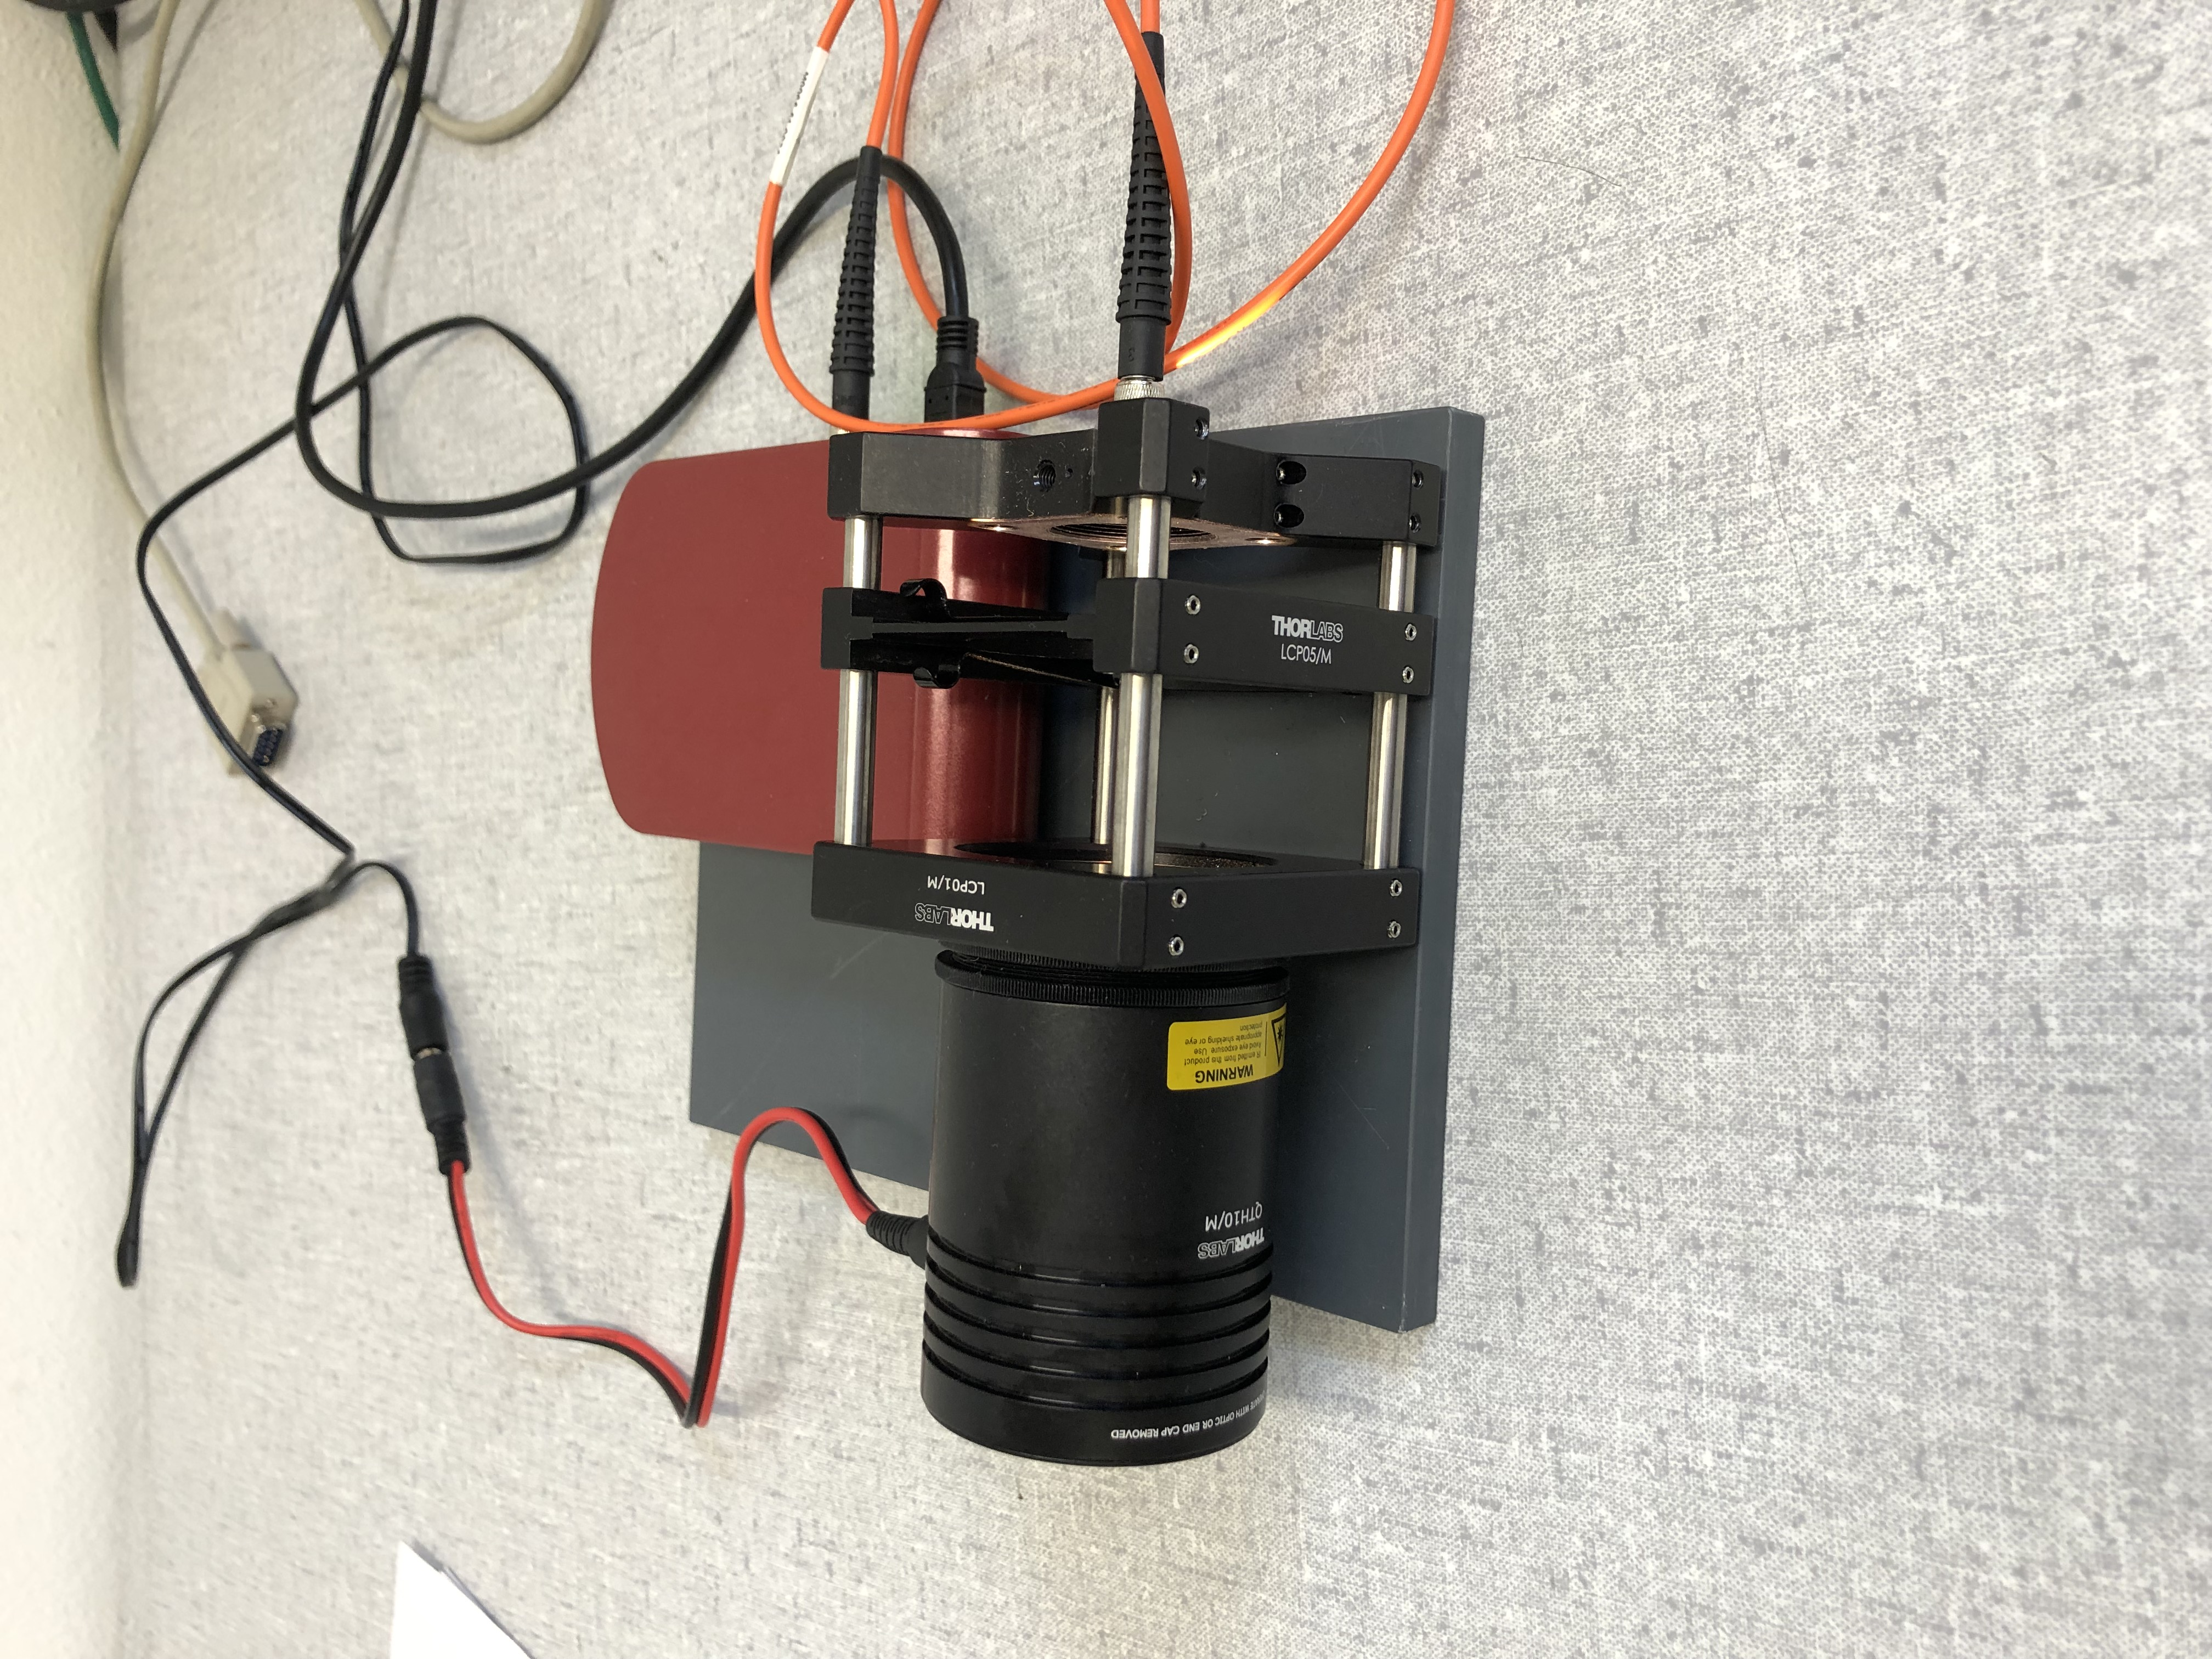
\includegraphics[angle=-90, width=\textwidth]{aufbau}
		\captionof{figure}{Versuchsaufbau}
		\label{fig:aufbau}
	\end{minipage}
\end{center}

\noindent Um die Funktionsweise eines Spektralphotometers zu verstehen, wird
zunächst der Aufbau eines Czerny-Turner Monochromators, wessen schematischer
Aufbau in folgender \autoref{fig:monoc} sichtbar ist, erklärt.

\begin{center}
	\begin{minipage}{0.5\textwidth}
		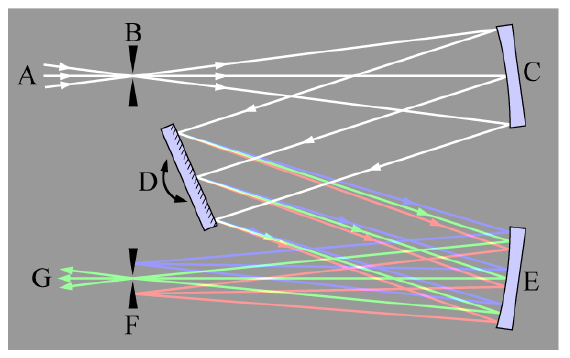
\includegraphics[width=\textwidth]{monoc}
		\captionof{figure}{Schematischer Aufbau eines Gittermonochromators \cite{wiki_gitterchromatorbild2020}}
		\label{fig:monoc}
	\end{minipage}
\end{center}

\noindent Das einfallende Licht A gelangt durch den Spalt B in die Apparatur.
Durch den sphärischen Spiegel C gelangt das Licht als parallele Strahlen auf
das Gitter D. Hier wird das Licht in die einzelnen Komponenten zerlegt, weil
die unterschiedlichen Wellenlängen verschieden stark gebeugt werden. Der zweite
sphärische Spiegel E bündelt die Lichtstrahlen wieder, sodass nur eine einzelne
Wellenlänge, also Farbeindruck, durch den Spalt bei F gelangt. Um die
Wellenlänge des Lichts G, welches den Monochromator verlässt, zu variieren,
kann das Gitter D geneigt werden \cite{demtroder2018ex2}.

\vspace{2mm}

\noindent Der Unterschied zum Monochromator ist, dass das Spektralphotometer
aufgrund einer Diodenzelle eine Vermessung der entsprechenden Spektren
ermöglicht.

\vspace{2mm}

\noindent Um die verschiedenen Messungen durchzuführen, wurden die Gegenstände,
welche in \autoref{fig:material} sichtbar sind, in die dafür vorgesehene
Halterung geklemmt.

\begin{center}
	\begin{minipage}{0.5\textwidth}
		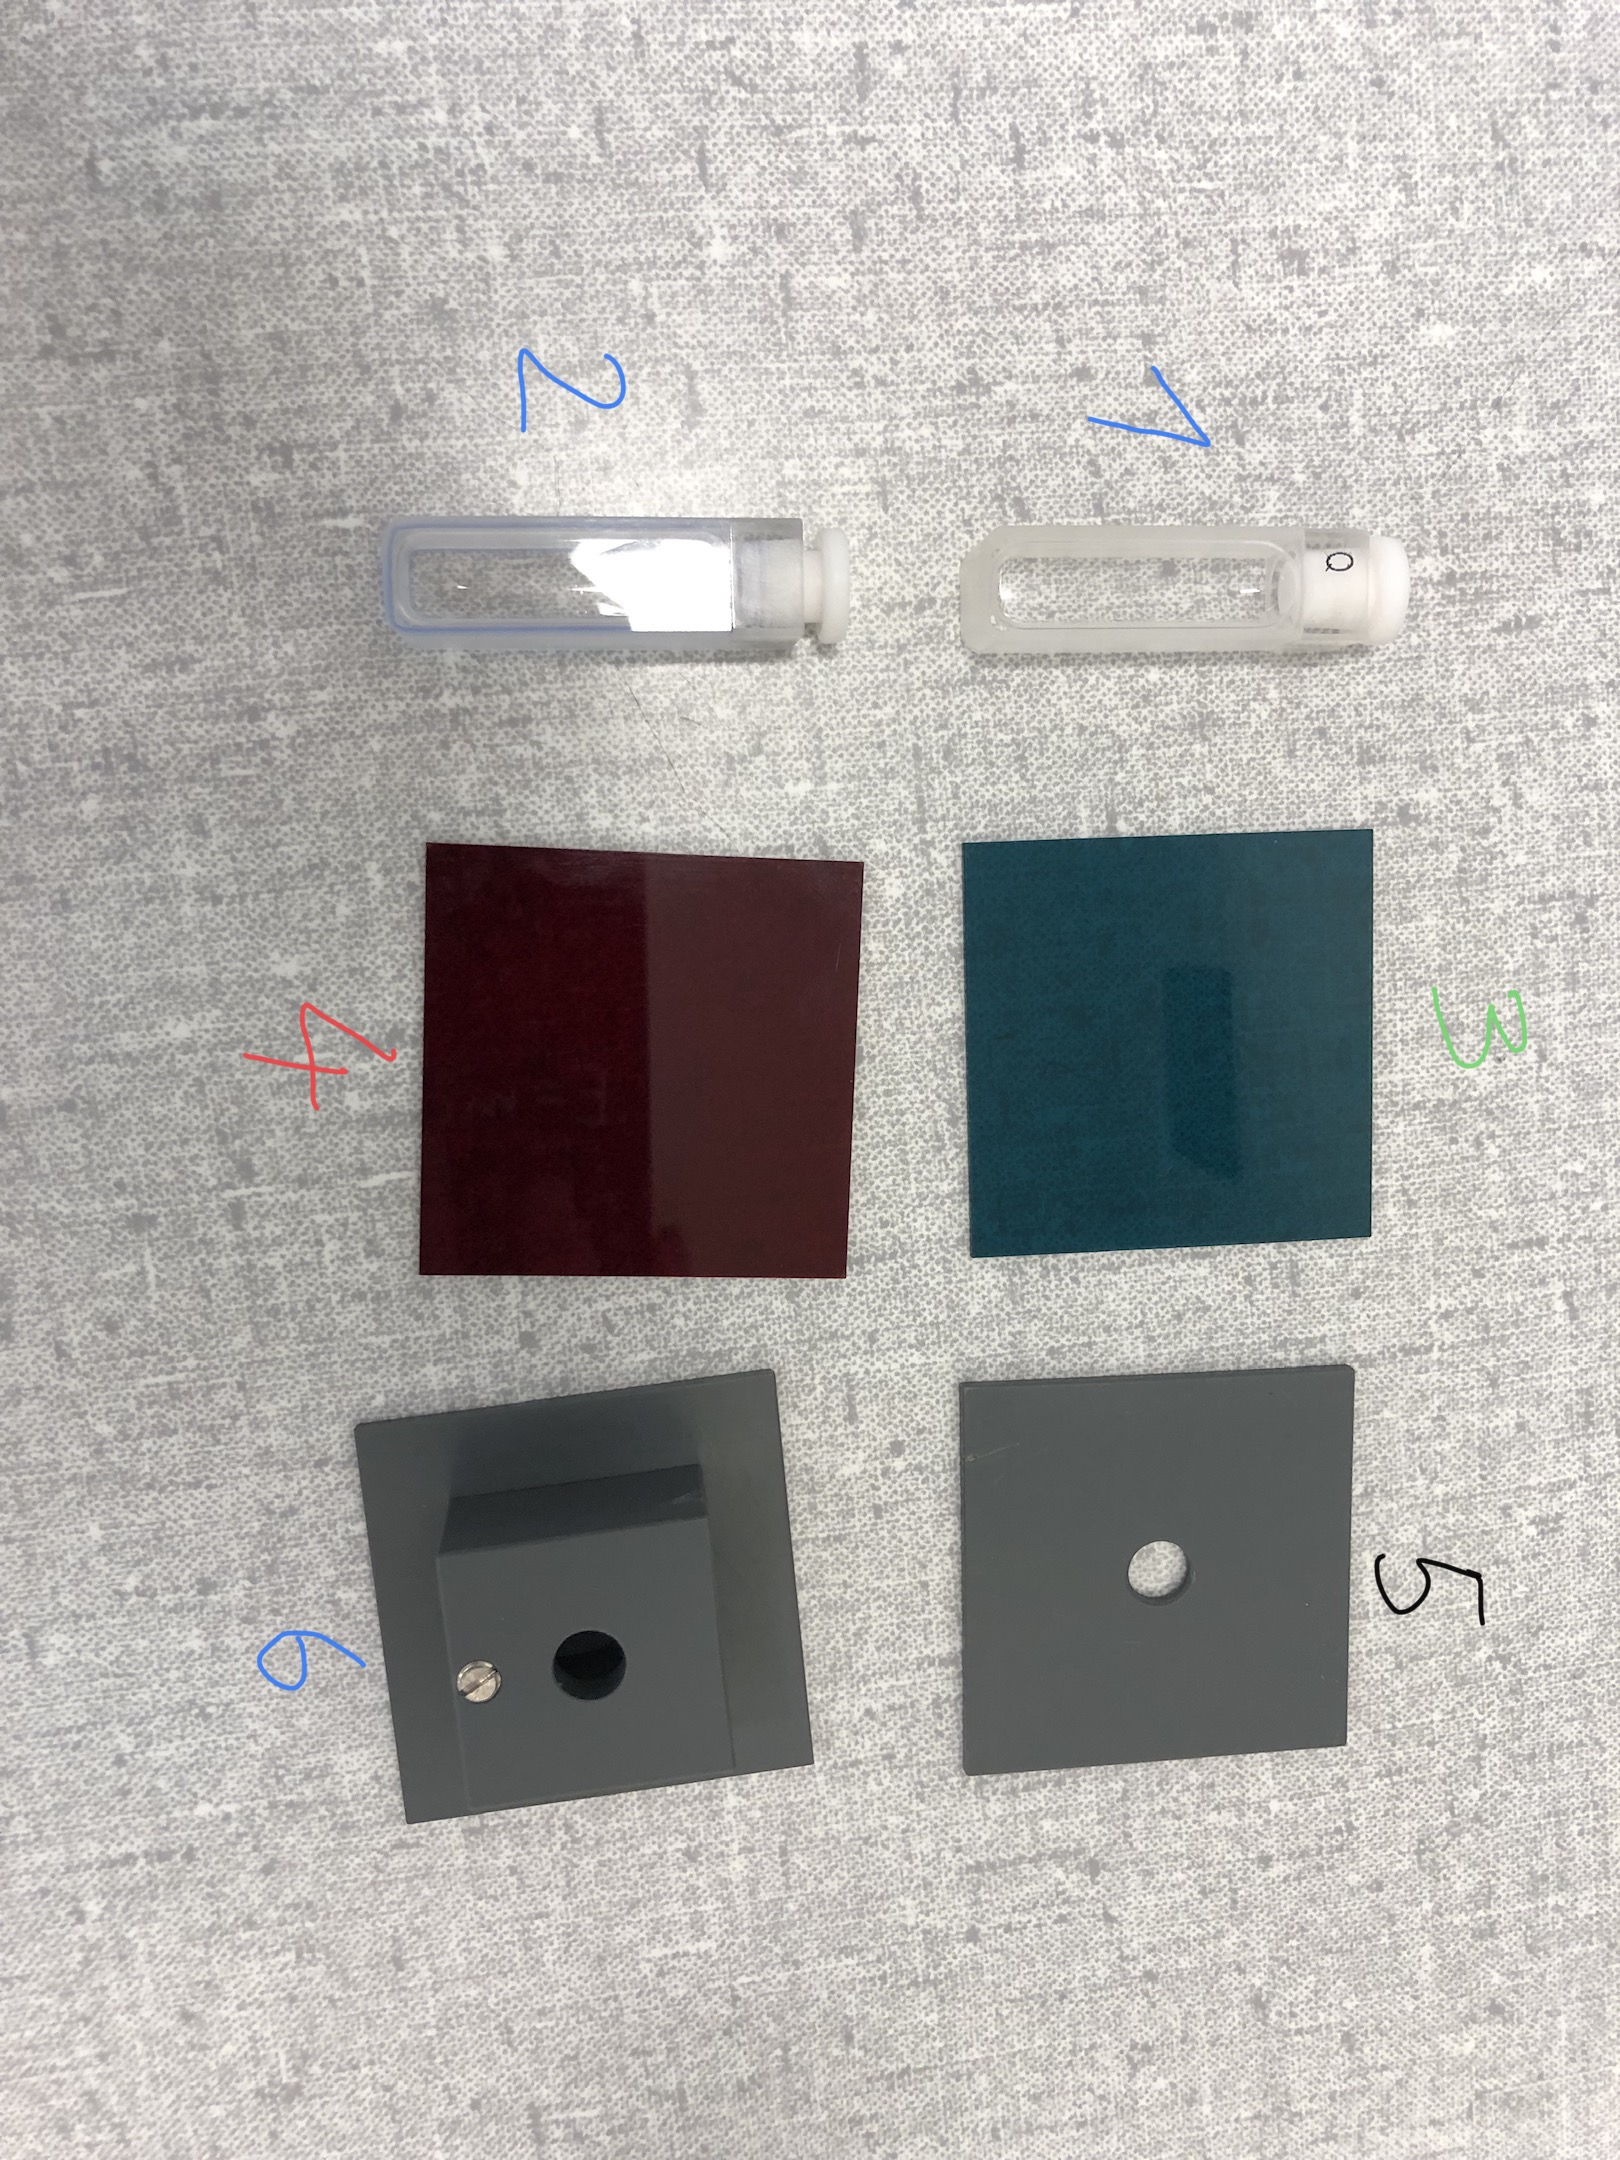
\includegraphics[angle=90, width=\textwidth]{material}
		\captionof{figure}{verwendete Materialien}
		\label{fig:material}
	\end{minipage}
\end{center}

\noindent Bei den Küvetten handelt es sich um die zu messende
Methylenblaulösung 2 und ein gleich großes, mit Wasser gefülltes, Fläschchen 1,
welches für die Referenzmessung verwendet wird. Die beiden Gefäße, werden
mithilfe der Halterung 6 in die Anordnung geschoben. Die bunten Plättchen in
Grün 3 und Rot 4, sowie die dünne Glasplatte, welche auf den Plastikteil 5
geklebt wurde, können direkt in die entsprechende Halterung gesteckt werden.

\newpage

\section{Geräteliste}

\noindent Für die Messungen wurden folgende Geräte verwendet:

\begin{table}[H]
	\captionof{table}{Verwendete Geräte }
	\begin{center}
		\begin{tabular}{|c|c|c|c|} \hline
			\textbf{Gerät}     & \textbf{Typ}                   & \textbf{Hersteller} \\ \hline

			Spektralphotometer & CCS200/M                       & Thorlabs            \\ \hline
			Halogenlampe       & QTH10/M                        & Thorlabs            \\ \hline
			Gestell            & LCP01/M                        & Thorlabs            \\ \hline
			Computersoftware   & SPLICCO                        &                     \\ \hline
			Farbfilter         & rot                            &                     \\ \hline
			Farbfilter         & grün                           &                     \\ \hline
			Küvette            & gefüllt mit Wasser             &                     \\ \hline
			Küvette            & gefüllt mit Methylenblaulösung &                     \\ \hline
			Halterung          & für Küvetten                   &                     \\ \hline
			Glasplatte         & befestigt auf Halterung        &                     \\ \hline
		\end{tabular}
	\end{center}
\end{table}




\section{Versuchsdurchführung \& Messergebnisse}\label{sec:Versuchsdurchführung}

\noindent Um den Versuch durchzuführen müssen zunächst die Wellenlängenbereiche
in der Computersoftware auf 400 bis 800 nm gestellt werden. Dies kann durch
einen Doppelklick auf die jeweiligen Werte der entsprechenden Achse
bewerkstelligt werden. Die ``Integration Time`` soll auf Werte zwischen 0,5 bis
2,0 ms gestellt werden, sodass das Spektrum der Lichtquelle den y-Achsenbereich
gut ausfüllt. Zuletzt muss noch ``Average scans`` auf den Wert 50 gestellt
werden.

\vspace{2mm}

\noindent Bei Änderungen des Umgebungslichts muss eine Hintergrundkorrektur
durchgeführt werden, indem der Knopf ``Save Background Correction`` betätigt
wird. Wichtig dabei ist, dass die Lichtquelle abgeblendet ist. Dies wird
dadurch erreicht, indem die Lampe abgedeckt wird. Die Lichtquelle darf
allerdings nicht einfach ausgeschaltet werden, da es einige Zeit dauert, bis
die Lampe konstant Licht von sich gibt und so die Messungen verfälscht werden
würden.

\subsection{Transmission und Extinktion}

\noindent Zunächst wird das Referenzspektrum gemessen, indem nur der
Versuchsaufbau ohne Zusätzliche Filter betrieben wird. Nun werden der Reihe
nach jeweils der rote, der grüne und schließlich beide Filter in die, dafür
vorgesehene Halterung geschoben und die entsprechenden Daten zur weiteren
Verarbeitung exportiert. In \autoref{fig:filter} ist sichtbar, wie ein
Farbfilter in die Halterung gesteckt wird.

\begin{center}
	\begin{minipage}{0.5\textwidth}
		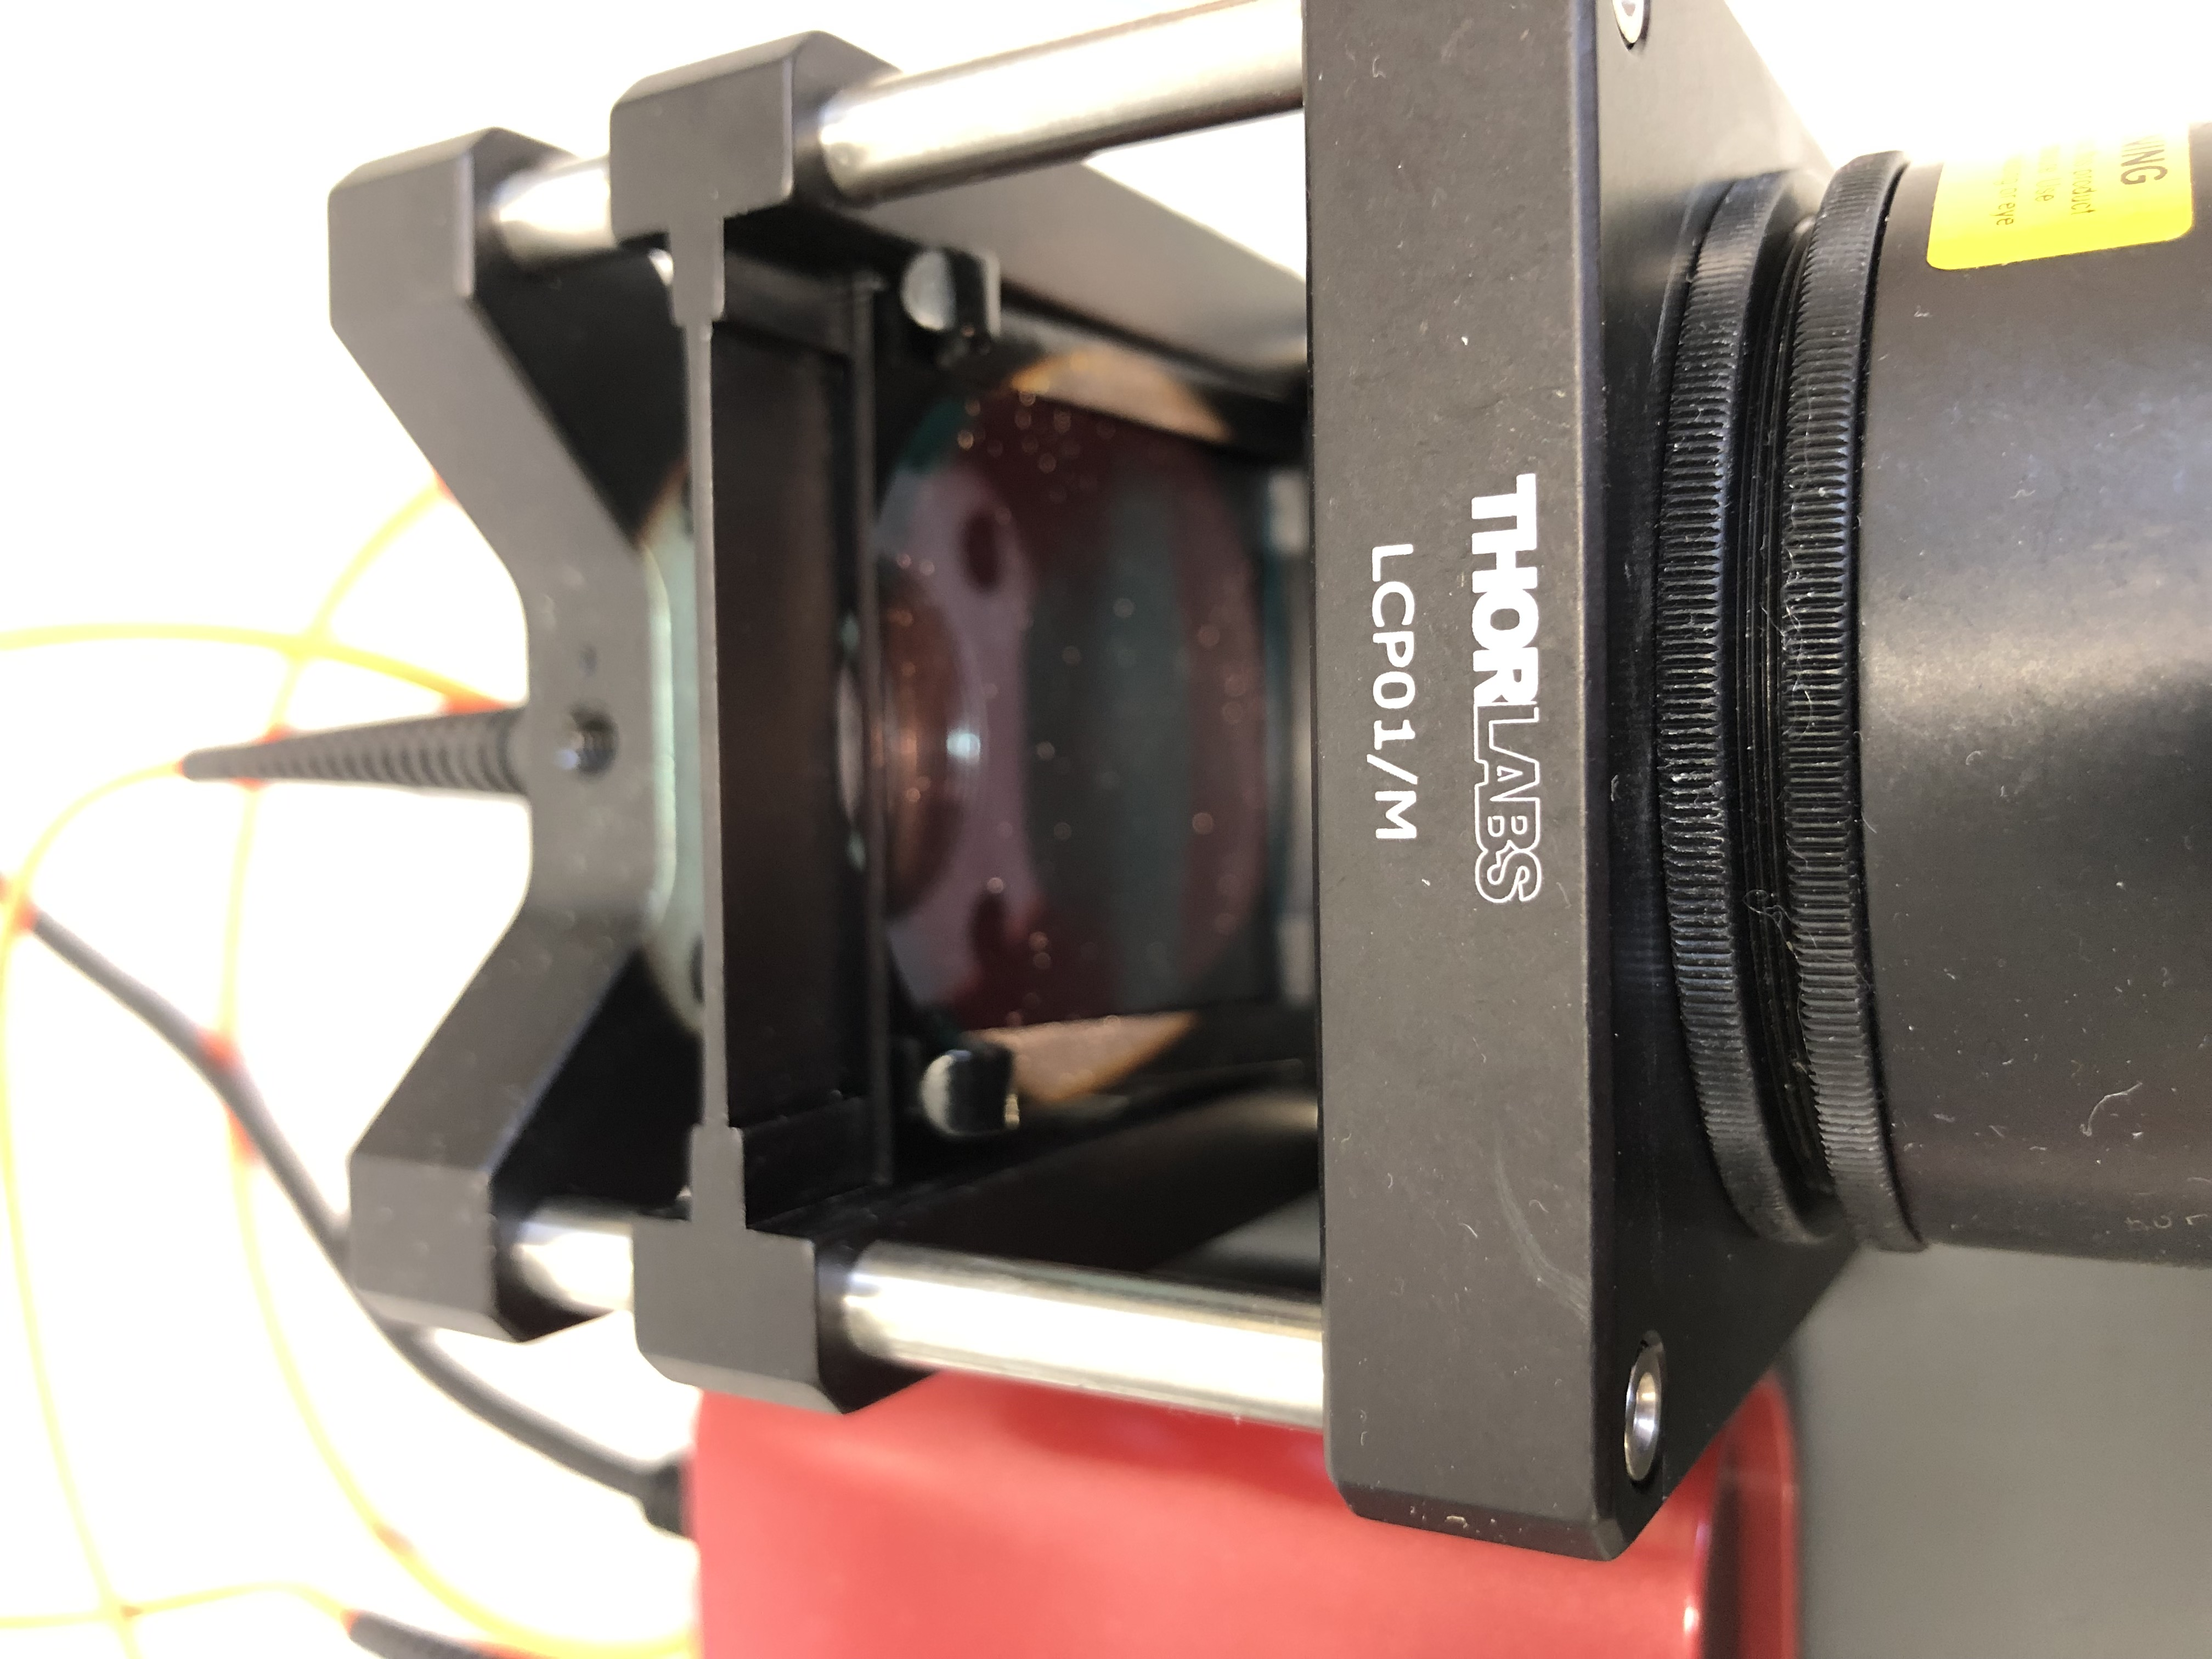
\includegraphics[ angle=-90,width=\textwidth]{filter}
		\captionof{figure}{in die Halterung gesteckter Farbfilter}
		\label{fig:filter}
	\end{minipage}
\end{center}

\vspace{2mm}

\noindent Ein Beispiel, wie die, vom Programm gemessenen Kurve aussieht ist in
\autoref{fig:gr} sichtbar. Hierfür wurde der grüne Filter verwendet.

\begin{center}
	\begin{minipage}{\textwidth}
		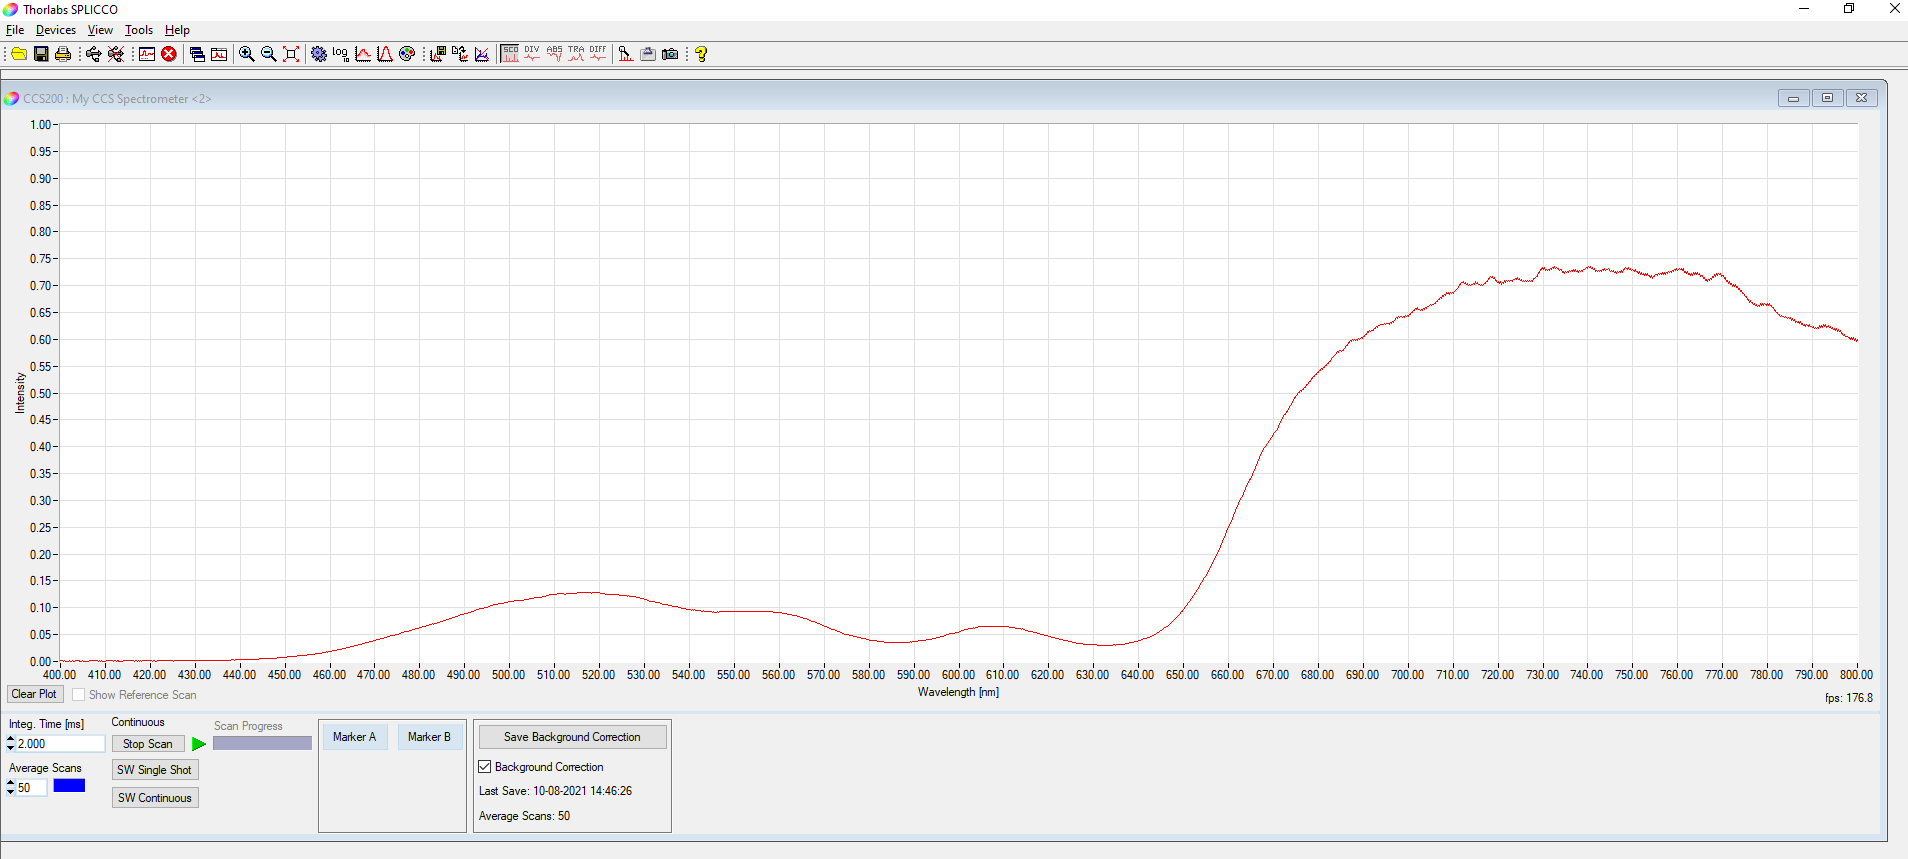
\includegraphics[ width=\textwidth]{gruen}
		\captionof{figure}{gemessene Kurve im Programm}
		\label{fig:gr}
	\end{minipage}
\end{center}

\noindent Um den statistischen Fehler, welcher beispielsweise durch Schwankungen der Hintergrundbeleuchtung oder Derartigen entsteht, möglichst gering zu halten, wurden alle Messungen 5 mal wiederholt. Dabei ist zu beachten, dass immer alle 4 Messungen abgeschlossen werden und dann die Wiederholung durchgeführt wird und nicht alle 5 Referenzmessungen direkt hintereinander durchgeführt werden. Durch dieses Vorgehen würden beispielsweise die eventuellen Änderungen des Umgebungslichts unbemerkt bleiben.

\subsection{Stoffmengenkonzentration der Methylenblaulösung}

\noindent Um die Stoffmengenkonzentration der Methylenblaulösung zu bestimmen, muss zunächst wieder eine Hintergrundkorrektur, wie bereits beschrieben, durchgeführt werden. Als Referenzmessung wird hier zunächst die mit Wasser gefüllte Küvette in die Halterung gesteckt, wie in \autoref{fig:kuv} sichtbar, und die entsprechende Messung durchgeführt.

\begin{center}
	\begin{minipage}{0.5\textwidth}
		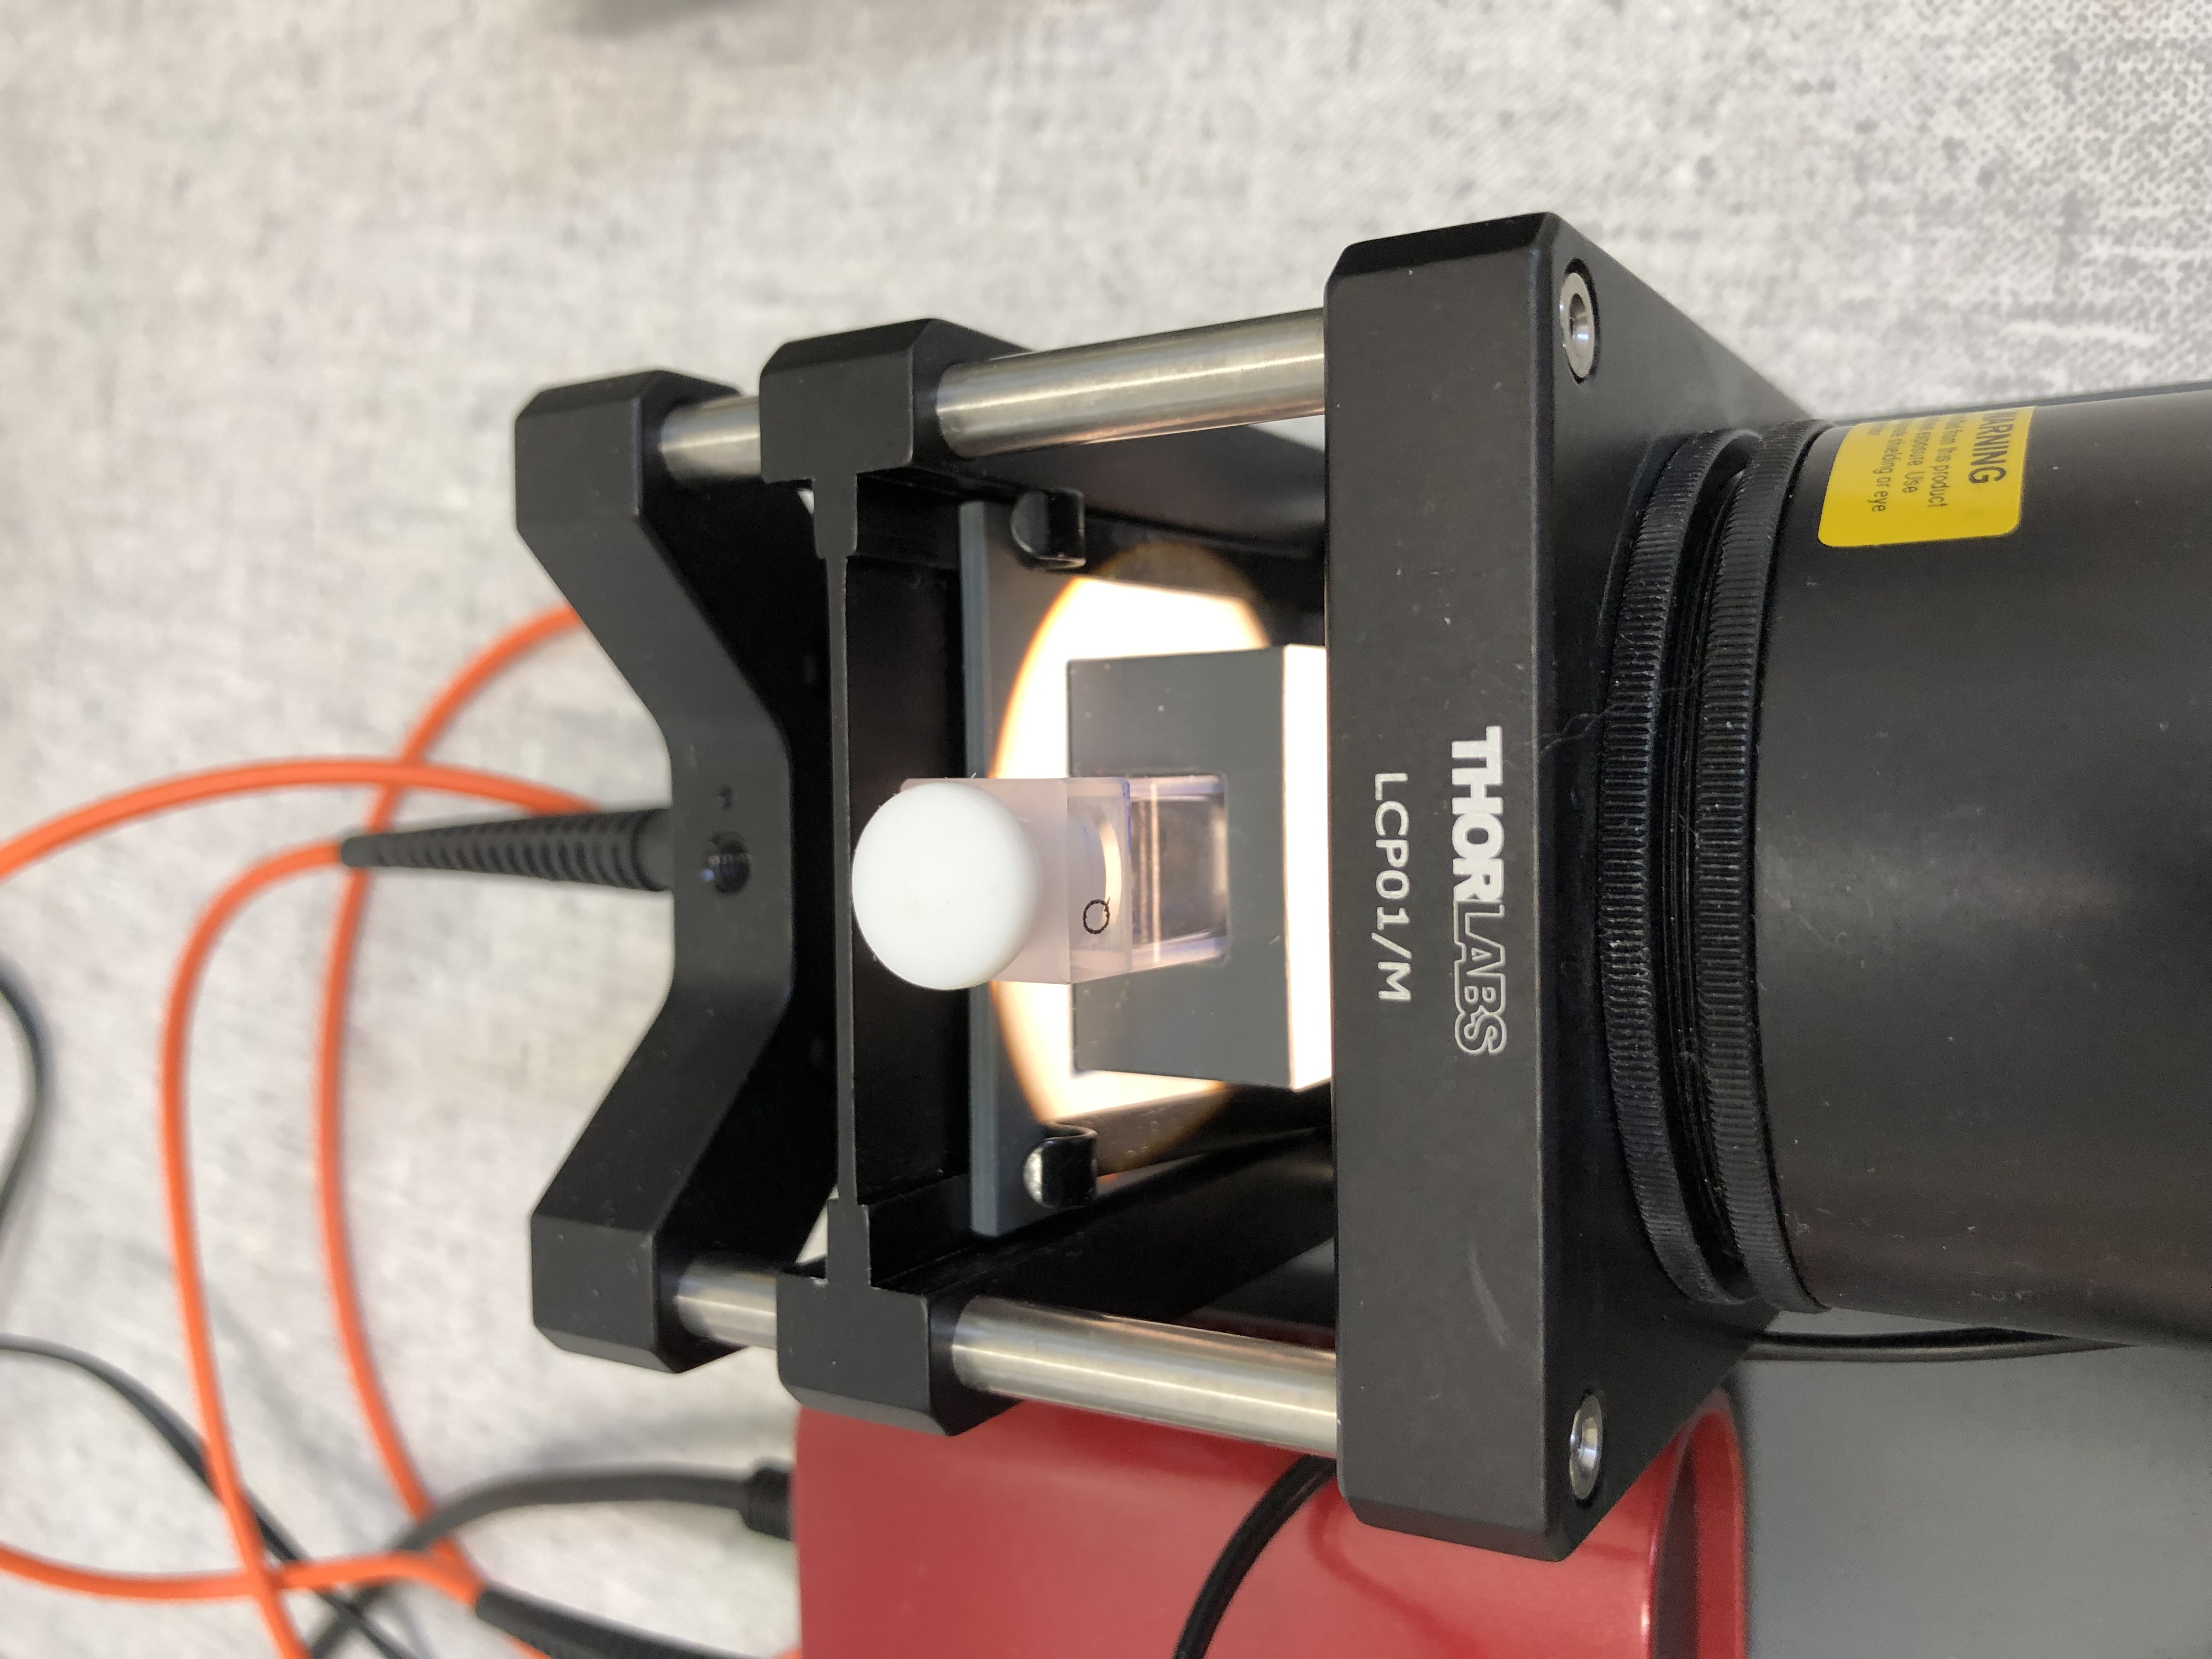
\includegraphics[ angle=-90,width=\textwidth]{kuv}
		\captionof{figure}{in die Halterung gesteckter Küvette}
		\label{fig:kuv}
	\end{minipage}
\end{center}

\noindent Nun werden die Referenzküvette durch die, mit dem Indikator gefüllte, ersetzt und die Daten wieder, wie bereits beschrieben,  exportiert. Auch dieser Versuch wird aus den selben Gründen, wie bereits zuvor, 5 mal wiederholt.

\subsection{Dicke der Glasplatte}

\noindent Um die Dicke der Glasplatte zu bestimmen, wurde der aufzulösende Bereich vergrößert, sodass auf der Abszisse ein Bereich von 665 bis 680 nm und auf der Ordinate eine Intensität von 0,7 bis 0,8 sichtbar wird. Der ausgewählte Bereich weist nun leichte Unebenheiten auf, wie in \autoref{fig:peaks_ohne} sichtbar.

\begin{center}
	\begin{minipage}{\textwidth}
		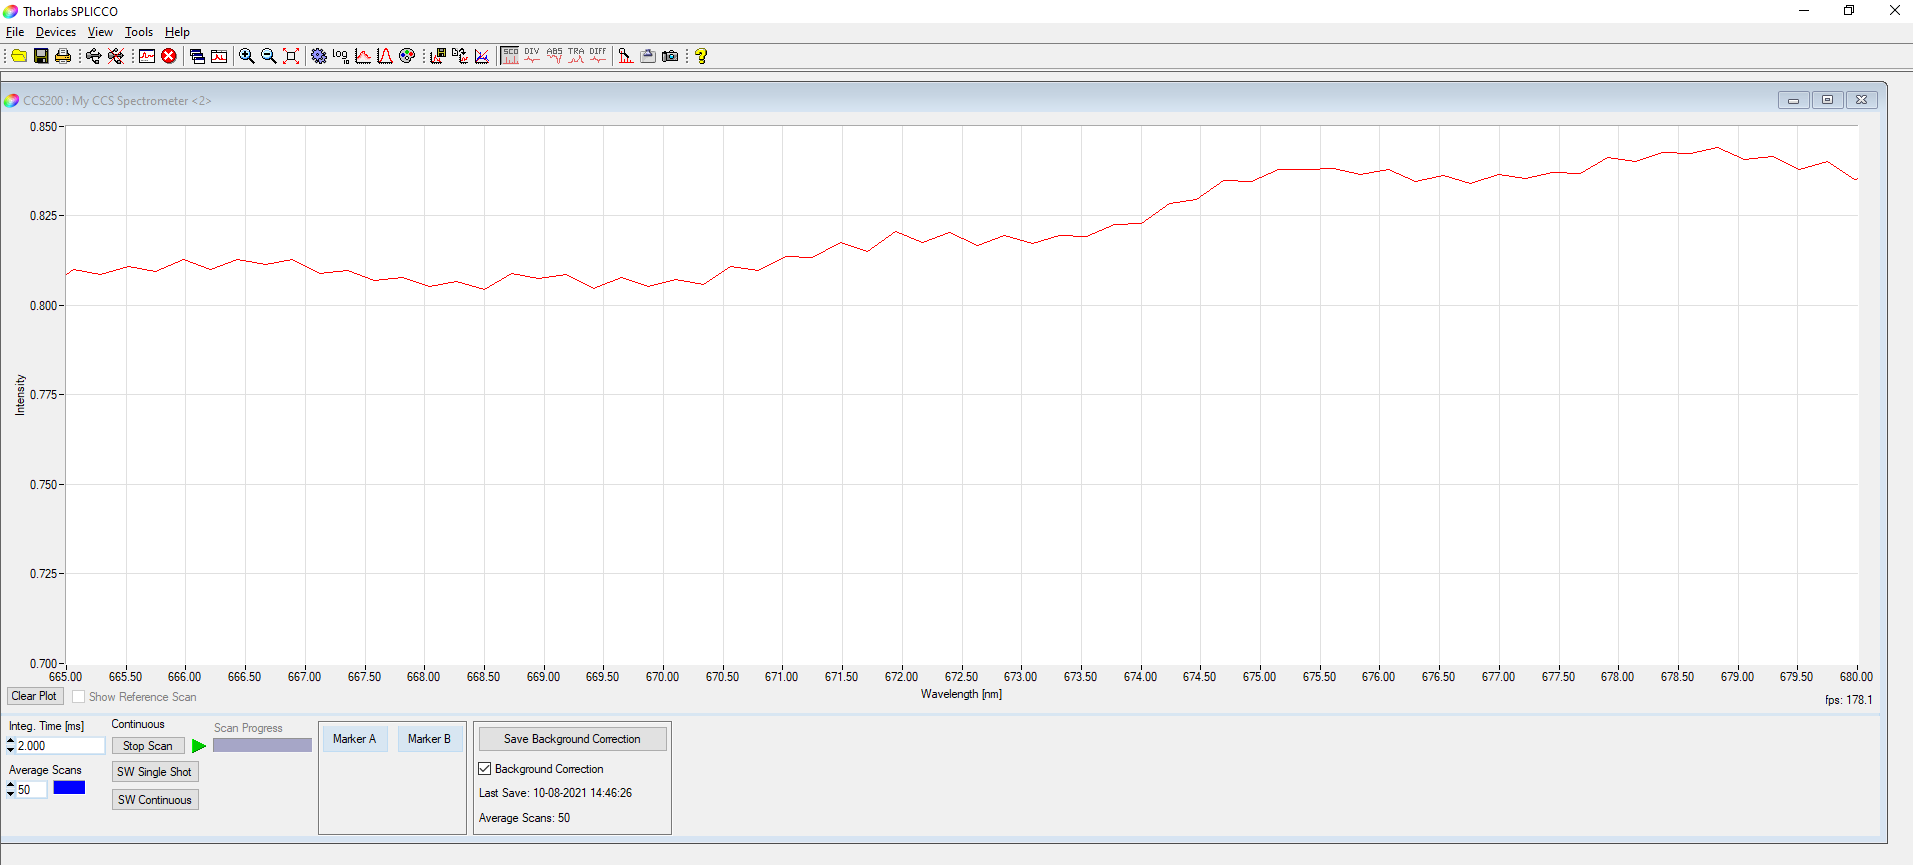
\includegraphics[ width=\textwidth]{peaks_ohne_neu}
		\captionof{figure}{Vergrößerter Bereich im Programm}
		\label{fig:peaks_ohne}
	\end{minipage}
\end{center}

\noindent Nun wird die Glasplatte eingeschoben, wie in \autoref{fig:loch} sichtbar, wodurch deutlich Peaks sichtbar werden, wie in \autoref{fig:peaks} sichtbar ist. Die Daten dieser Peaks müssen nun ermittelt und ausgewertet werden.

\begin{center}
	\begin{minipage}{\textwidth}
		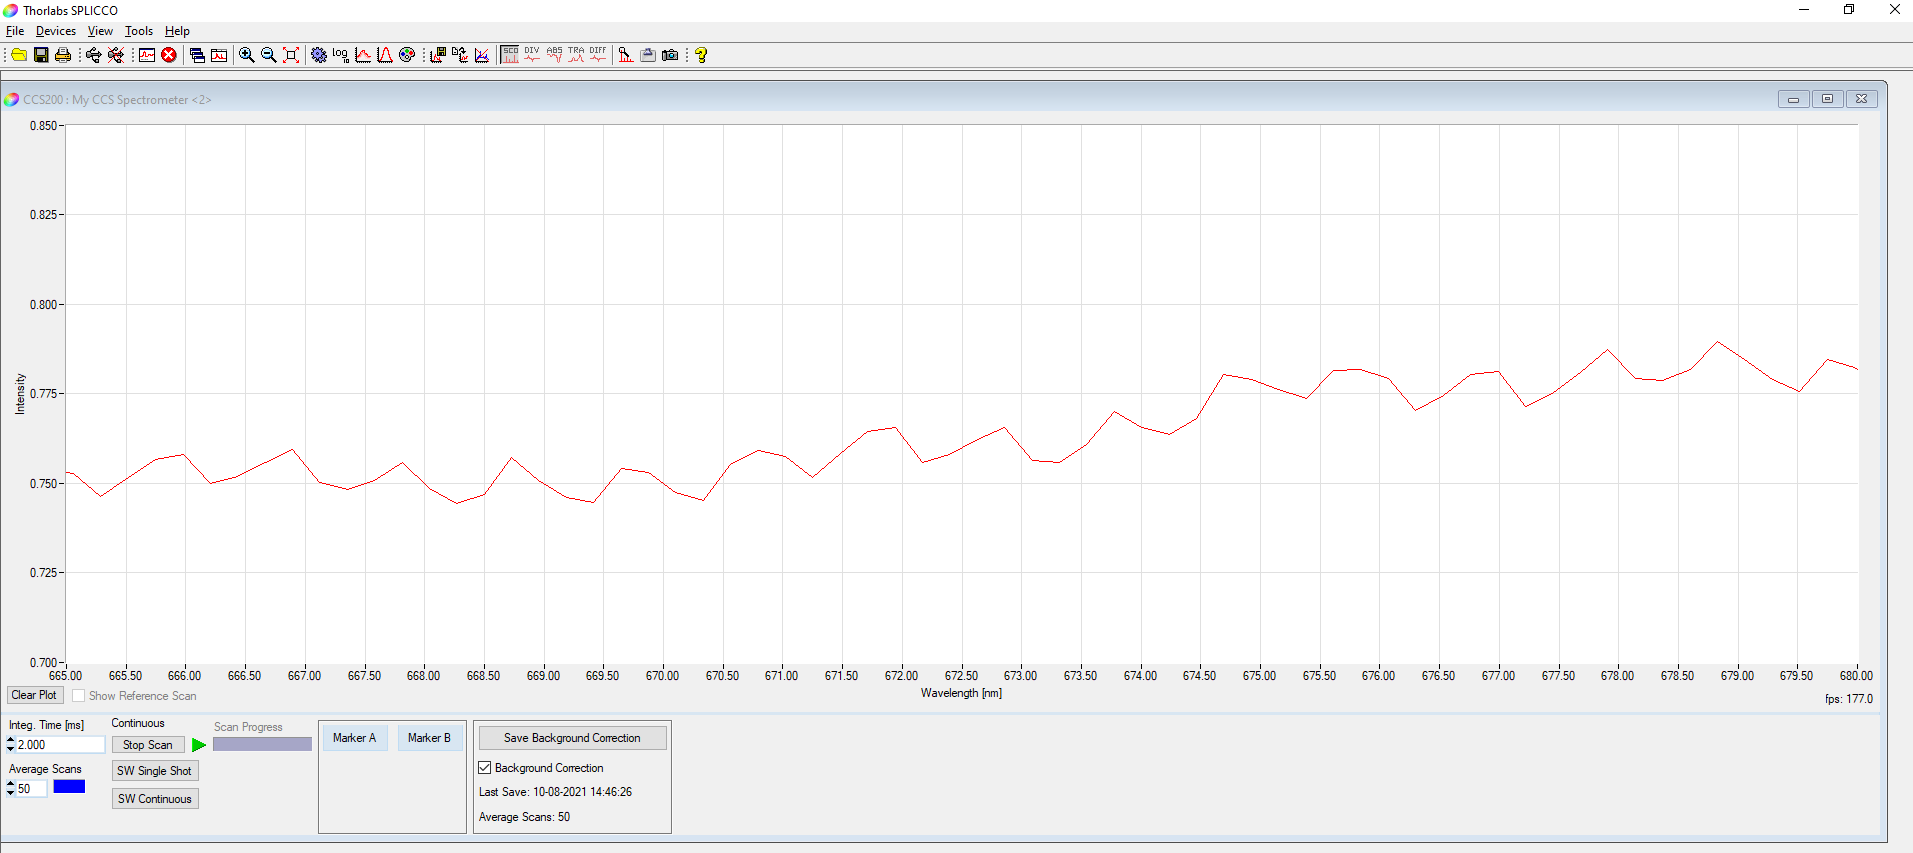
\includegraphics[ width=\textwidth]{peaks_neu}
		\captionof{figure}{Vergrößerter Bereich im Programm mit eingeschobener Glasplatte}
		\label{fig:peaks}
	\end{minipage}
\end{center}

\begin{center}
	\begin{minipage}{0.5\textwidth}
		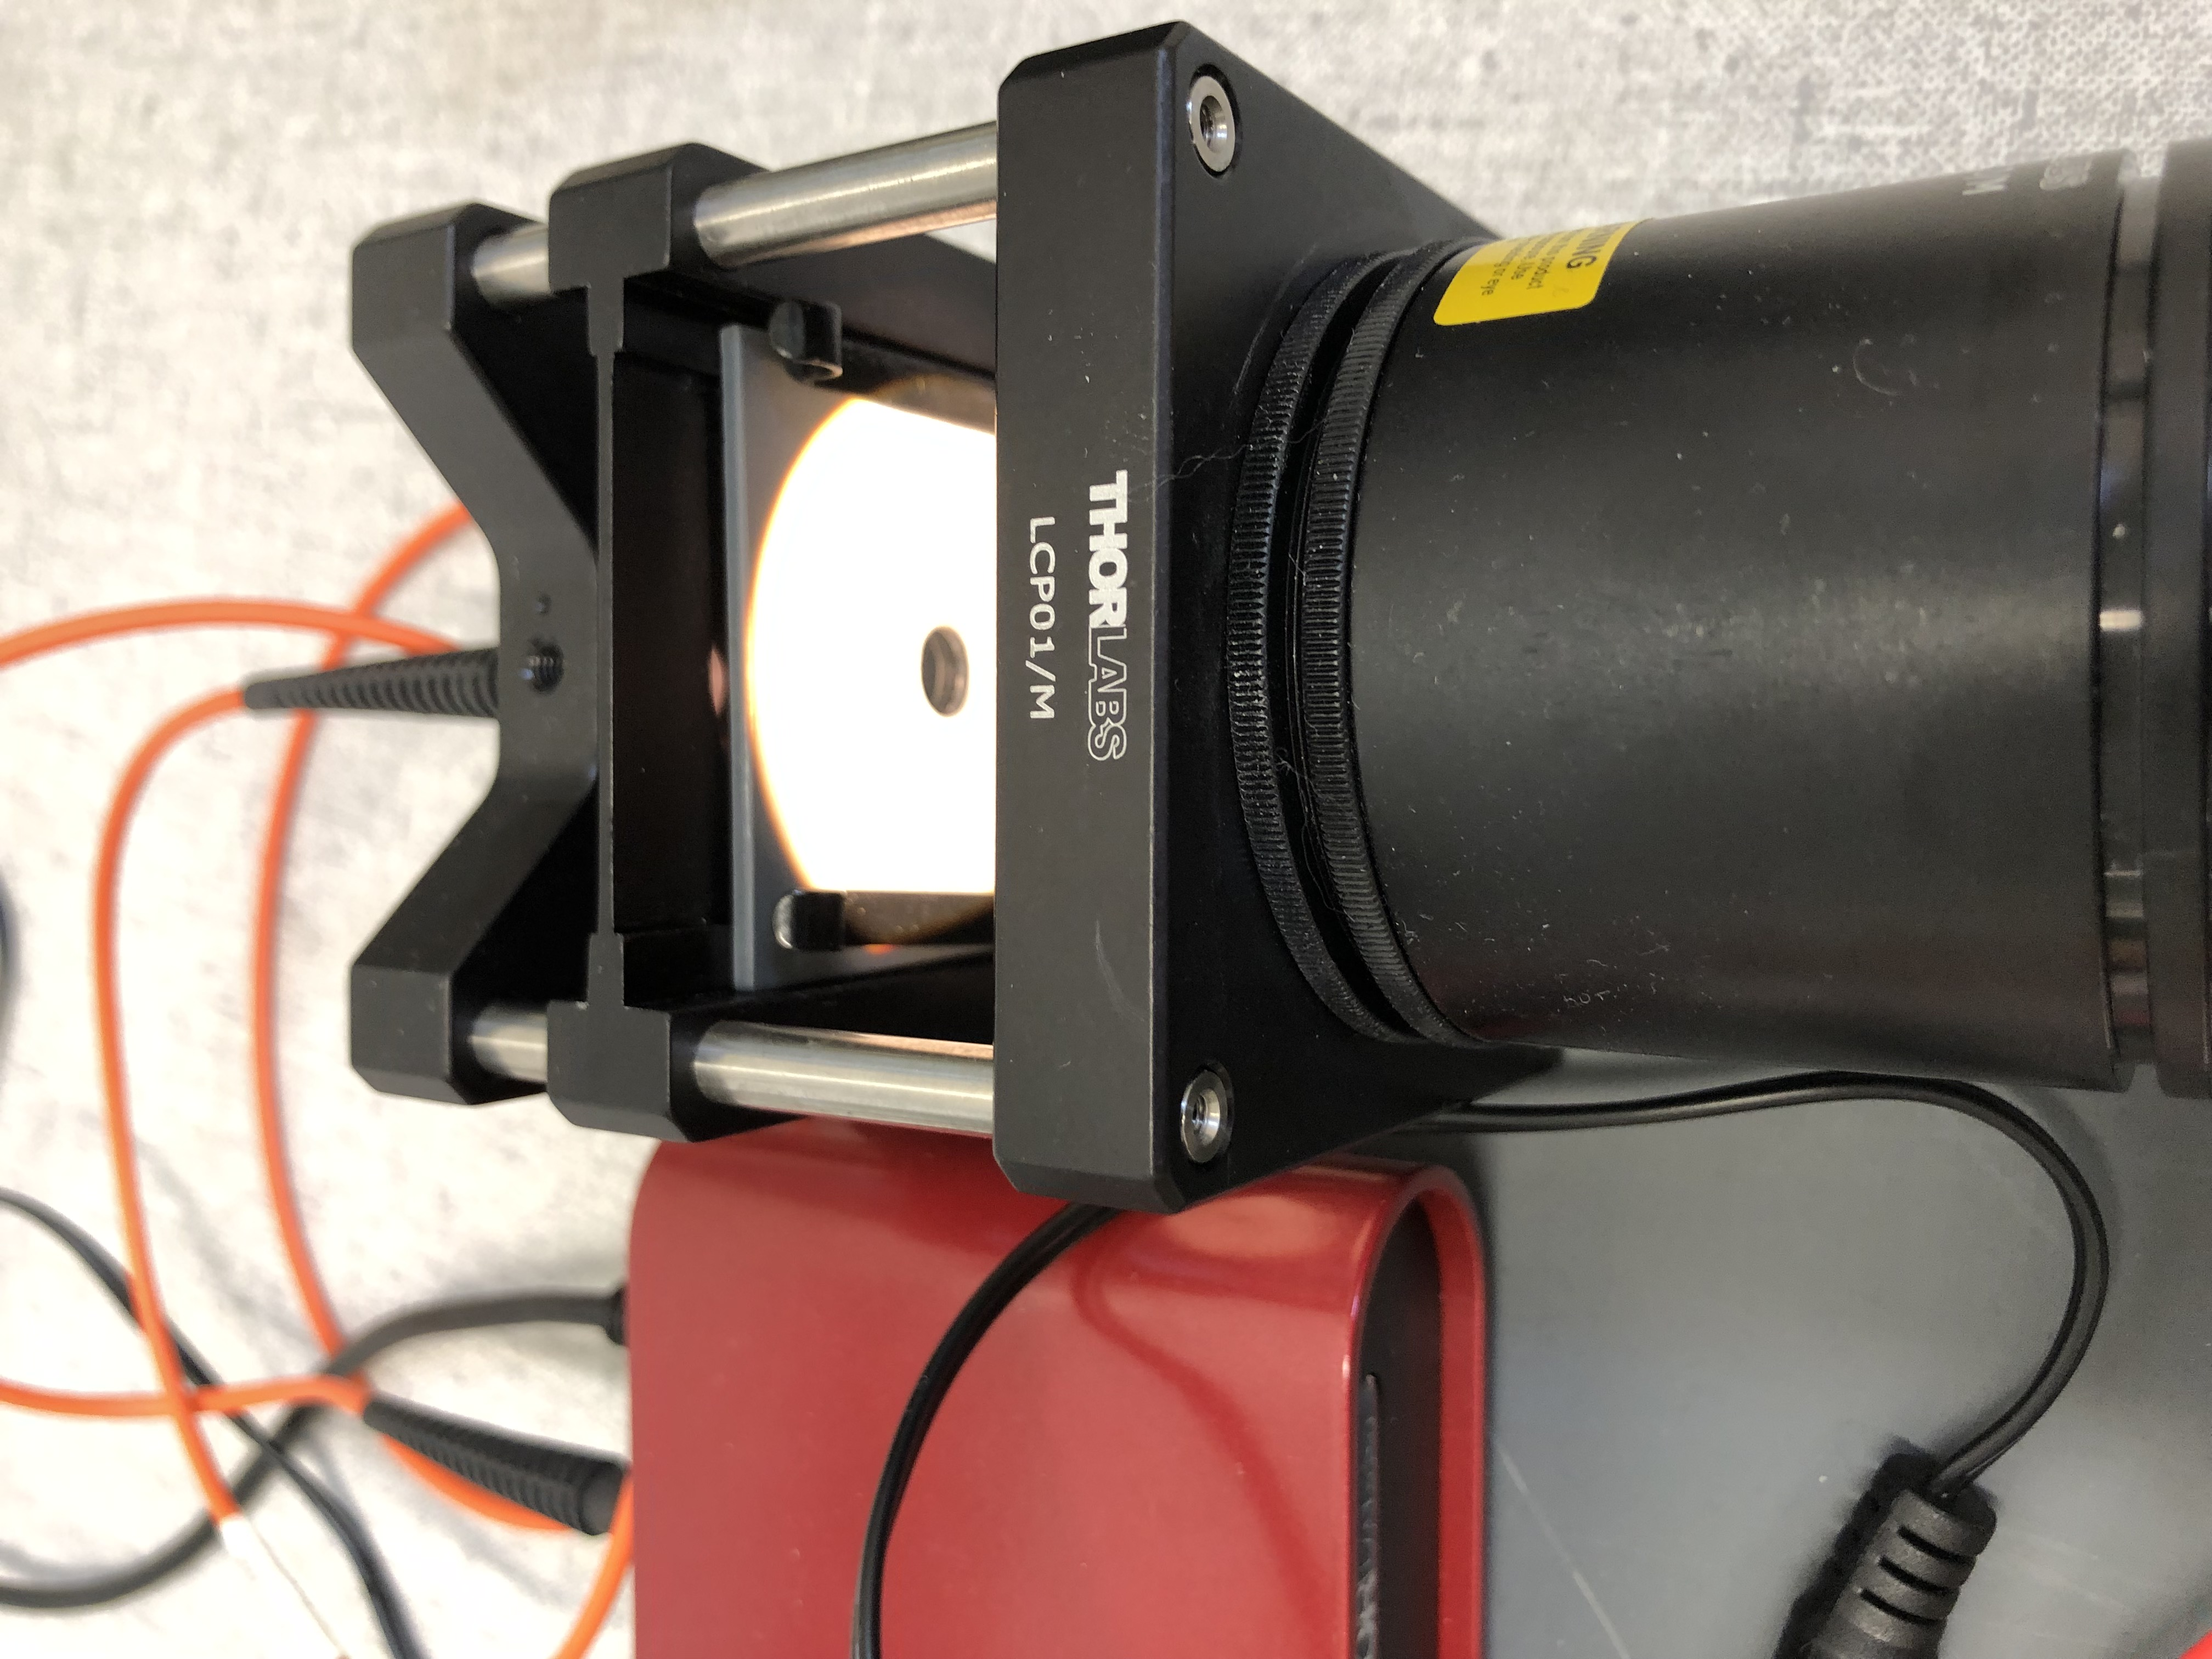
\includegraphics[ angle=-90,width=\textwidth]{loch}
		\captionof{figure}{in die Halterung gesteckter Glasplatte}
		\label{fig:loch}
	\end{minipage}
\end{center}

\section{Auswertung}

\subsection{Transmission und Extinktion}

Werden nun die Referenzwerte der Intensität der Halogenlampe im Verhältnis zu den gefilterten Intensitäten gebildet, erhält man die jeweiligen Transmissionen. Zudem wird die Extinktion aus dem Logarithmus des inversen Intensitätsverhältnisses nach \autoref{eq:extinktion} bestimmt. Die Ergebnisse sind in folgenden 4 Abbildungen ersichtlich.

\vspace{2mm}

\noindent Wie bereits in \nameref{sec:Versuchsdurchführung} erwähnt, wurden die
Messungen 5 mal wiederholt und anhand dieser Daten eine statistische
Normalverteilung, welche ebenfalls im Graphen anhand der blauen Kreuzze
ersichtlich ist, für den Fehler angenommen. Der entsprechende Fehler, der durch
standard error bestimmt worden ist, wurde mittels student-t Verteilung
angepasst.


%grün ...4

\begin{center}
	\begin{minipage}{0.65\textwidth}
		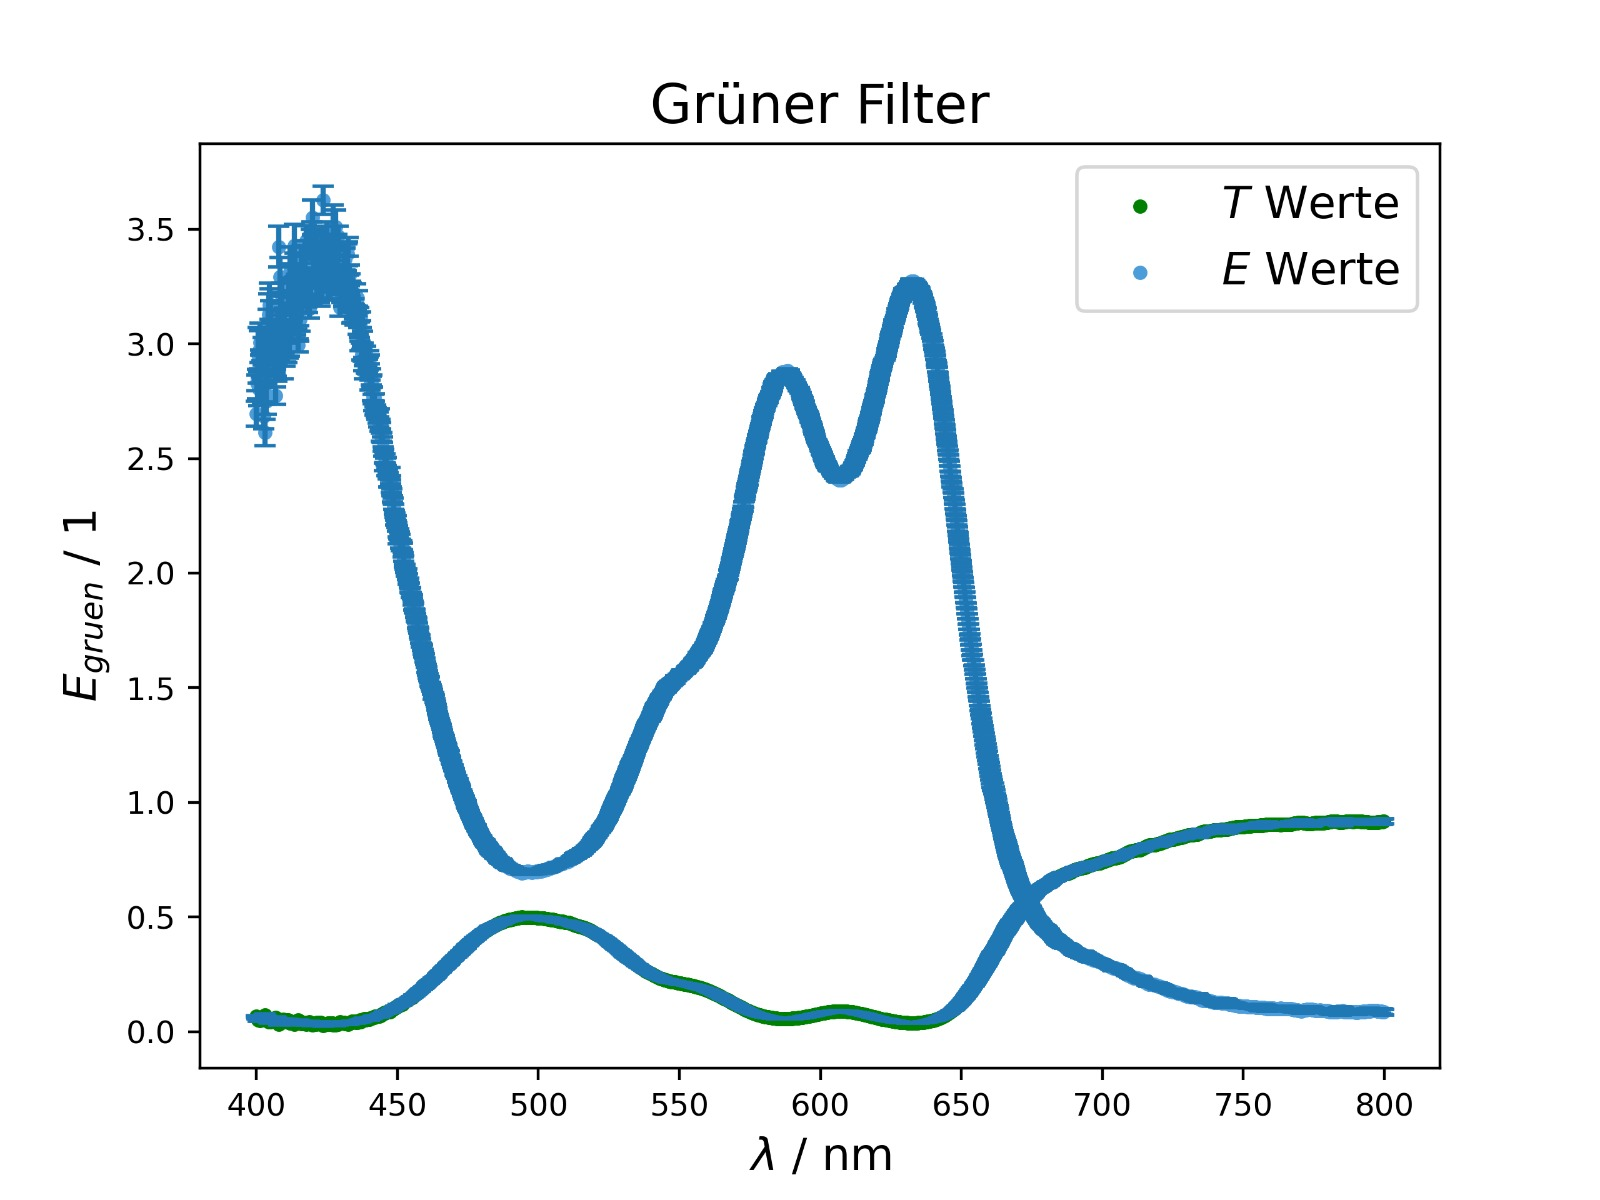
\includegraphics[width=\textwidth]{gruen_f}
		\captionof{figure}{Extinktion und Transmission bei der jeweiligen Wellenlänge mit grünem Filter}
		\label{fig:gruen_f}
	\end{minipage}
\end{center}

\begin{center}
	\begin{minipage}{0.65\textwidth}
		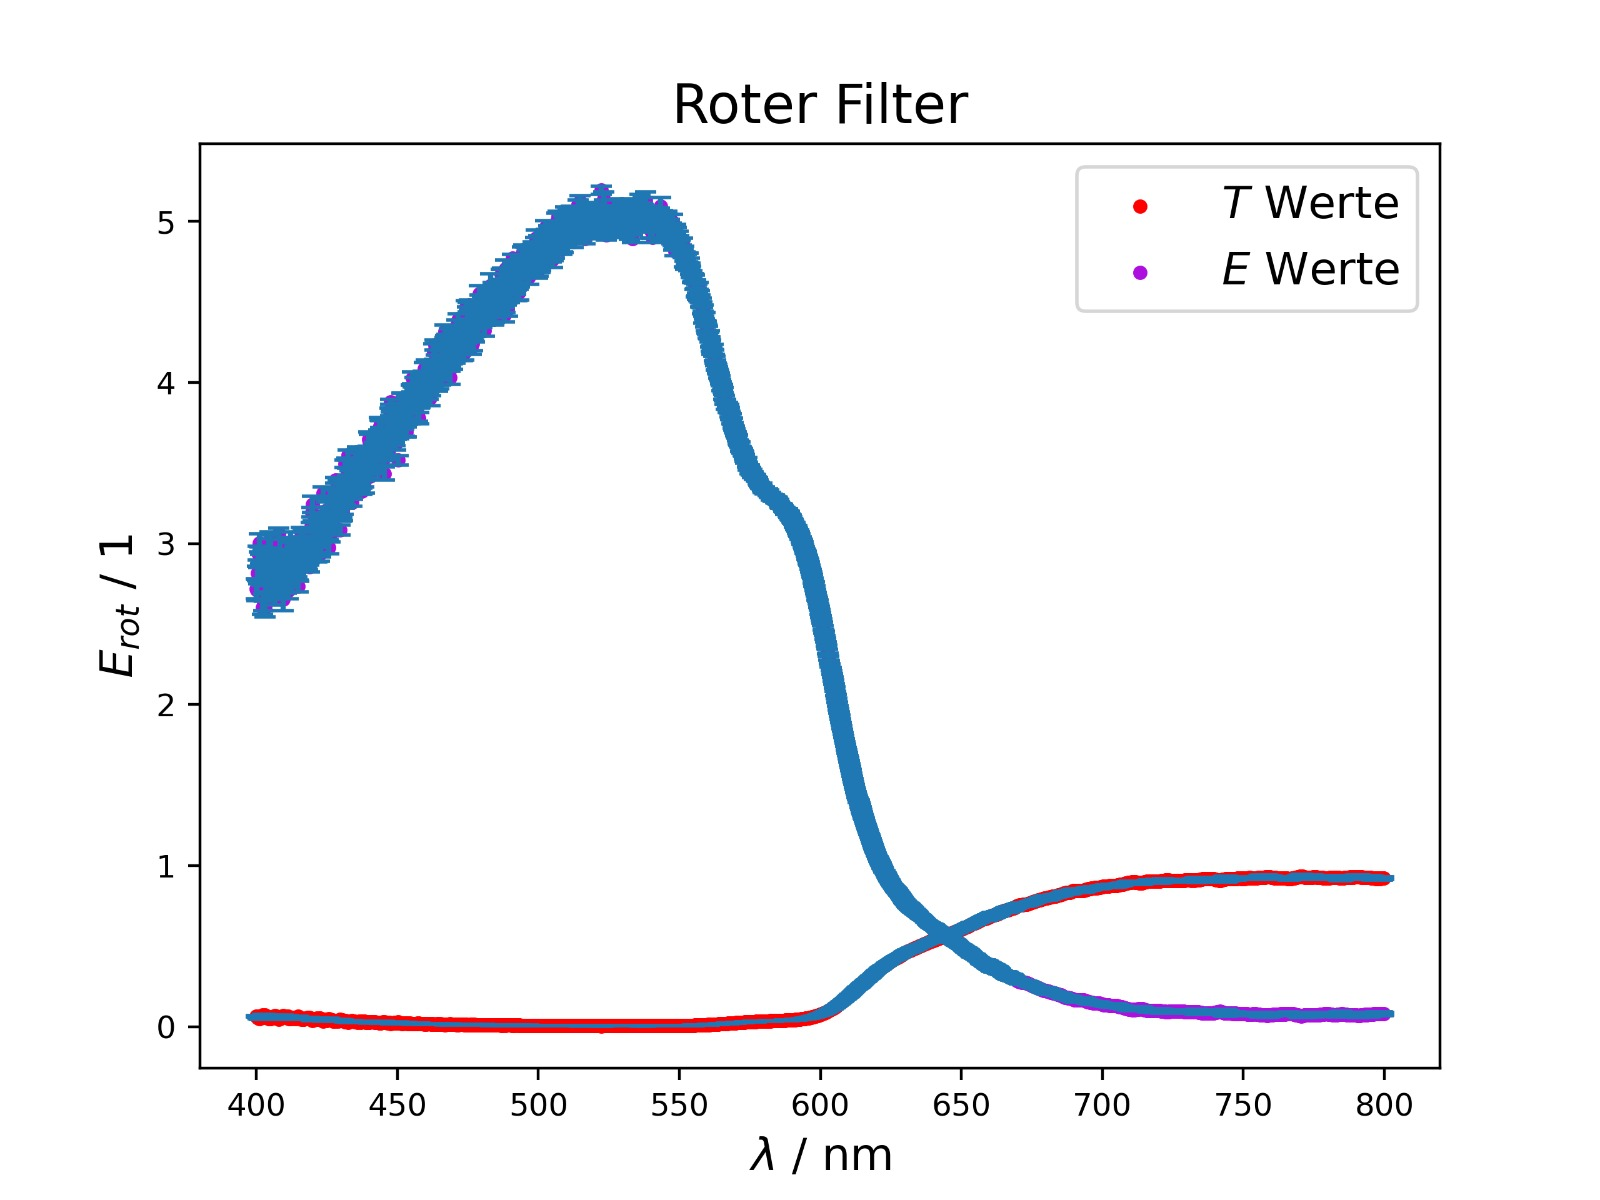
\includegraphics[width=\textwidth]{rot}
		\captionof{figure}{Extinktion und Transmission bei der jeweiligen Wellenlänge mit roten Filter}
		\label{fig:rot}
	\end{minipage}
\end{center}

\begin{center}
	\begin{minipage}{0.65\textwidth}
		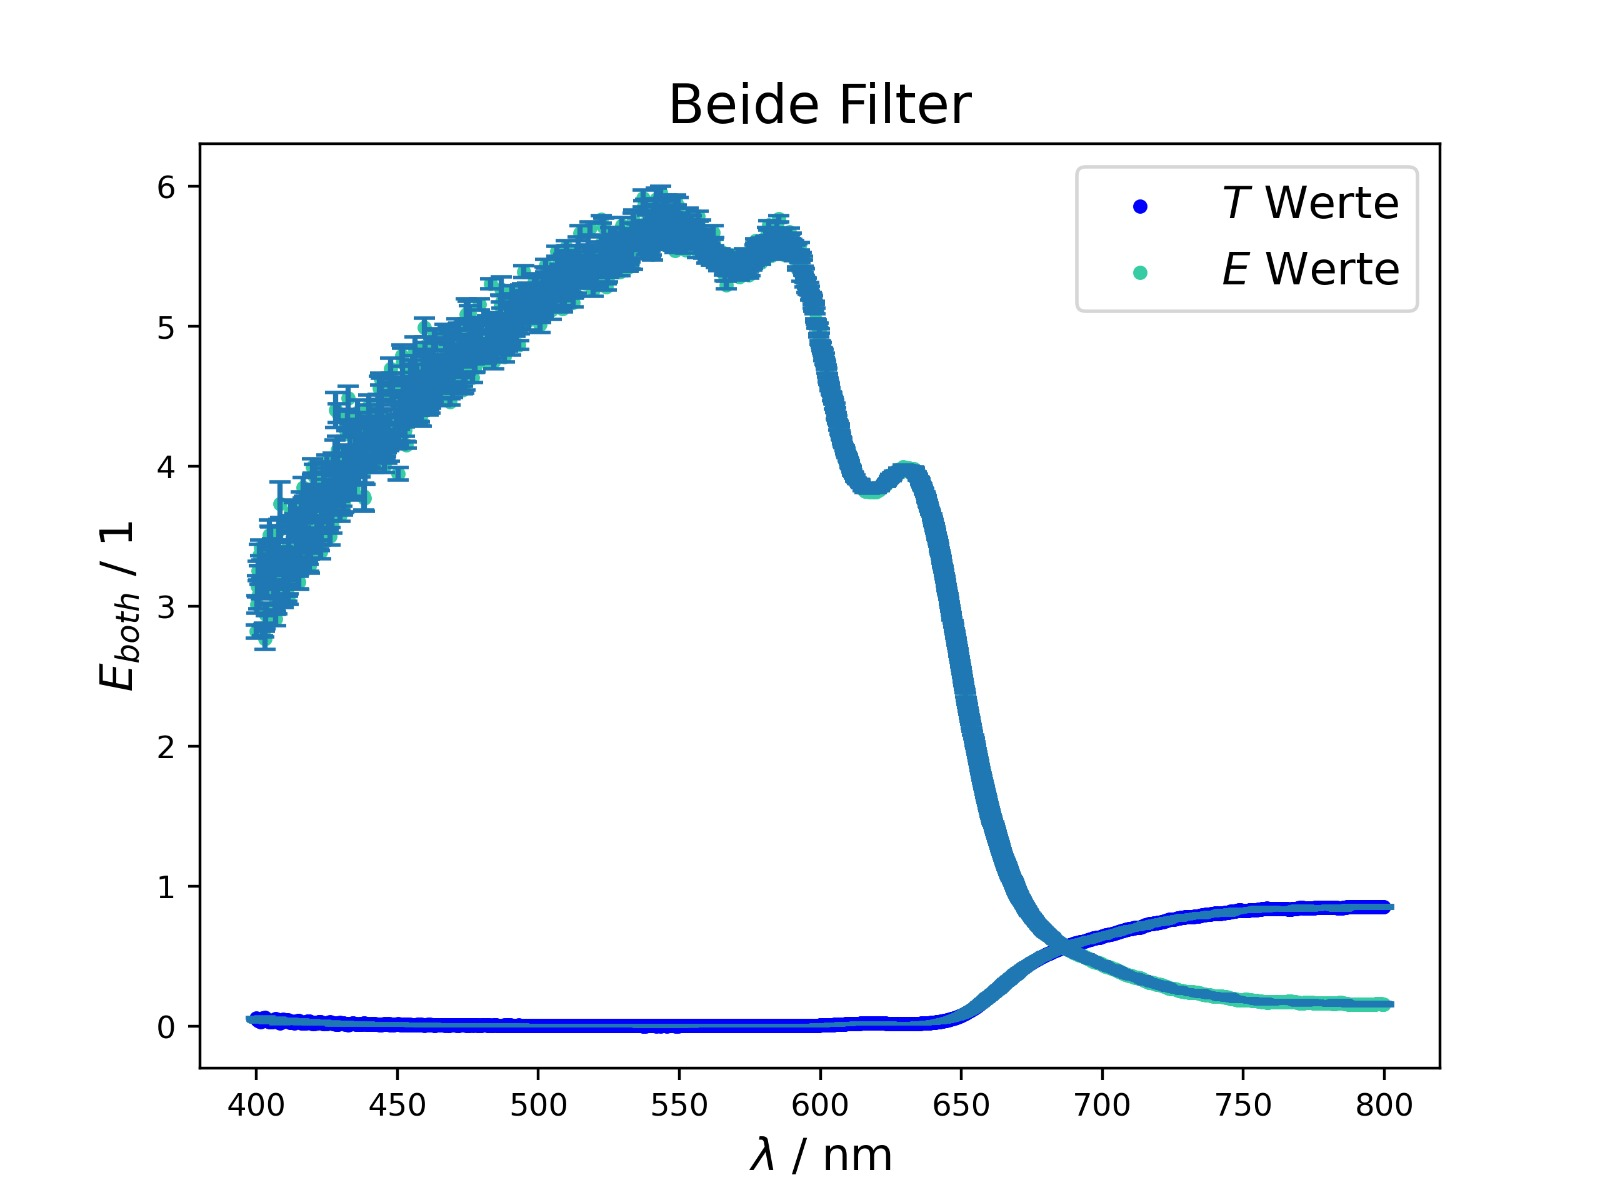
\includegraphics[width=\textwidth]{beide}
		\captionof{figure}{Extinktion und Transmission bei der jeweiligen Wellenlänge mit beiden Filtern}
		\label{fig:beide}
	\end{minipage}
\end{center}

\begin{center}
	\begin{minipage}{0.65\textwidth}
		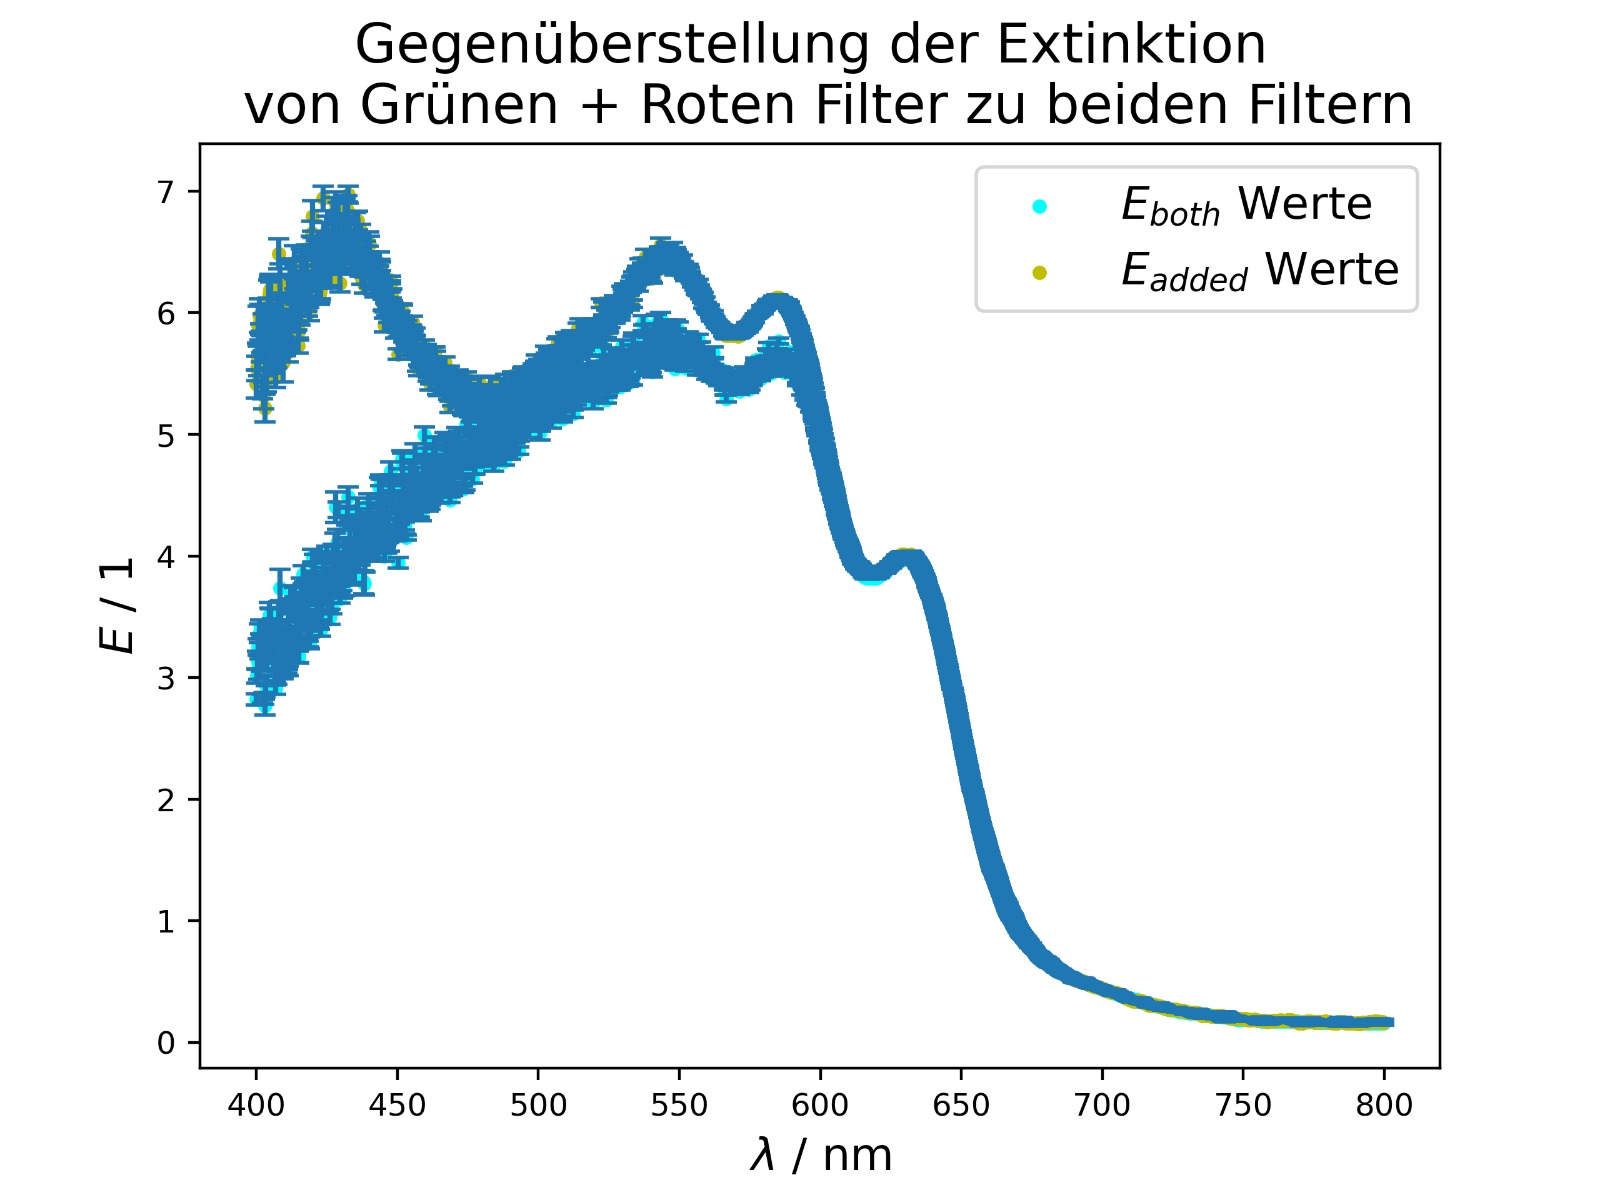
\includegraphics[width=\textwidth]{gegenuberst}
		\captionof{figure}{Gegenüberstellung der Extinktion bei beiden Filtern ($E_{both}$) und der Addition von beiden separaten Filtern ($E_{added}$)}
		\label{fig:geg}
	\end{minipage}
\end{center}

\newpage

\subsection{Stoffmengenkonzentration der Methylenblaulösung}

Aus den 5 mal gemessenen Datensätzen werden die Wellenlängen von \SI{664}{\nm} extrahiert und das Verhältnis der Intensitäten bei der Wellenlänge bestimmt um die Extinktion nach \autoref{eq:extinktion} zu bestimmen. Für die Intensitäten ergeben sich dabei folgende Werte:

\begin{align*}
	I_W = \SI{0.741(5)}{\watt\per\meter\squared} \\
	I_M = \SI{0.737(3)}{\watt\per\meter\squared}
\end{align*}

\noindent Unter Verwendung der Werte des dekadischen Extinktionskoeffizienten
$\varepsilon$ = \SI{77790}{\liter\per\mol\per\cm}, bei einer Wellenlänge 664
nm, der Schichtdicke der Lösung in der Küvette \SI{10}{\mm} und der Folgenden
\autoref{eq:konzentr} lässt sich die molare Konzentration $c$ berechnen.

\begin{equation}
	c = \frac{E(\lambda)}{\varepsilon d}
	\label{eq:konzentr}
\end{equation}

\noindent Daher ergibt sich für die Konzentration $c$ folgender Wert:

\begin{align*}
	c =  \SI{3.1(2)e-8}{\mol\per\liter}
\end{align*}




\subsection{Dicke der Glasplatte}



\noindent Zunächst muss die \autoref{eq:opweg} auf die Wellenzahl $\nu = \frac{1}{\lambda} $ umgeformt werden, wodurch folgender Ausdruck entsteht:

\begin{equation}
	\nu = \frac{k}{2n_P d} , \quad k\in \mathbb{Z}
	\label{eq:wellenz}
\end{equation}

\noindent Da nicht sichergestellt ist, dass das k null ist, wird noch eine Konstante $\kappa$ addiert, um den möglichen y-Versatz zu berücksichtigen.

\begin{equation}
	\nu = \frac{k}{2n_P d} + \kappa , \quad k\in \mathbb{Z}, \, \kappa \in \mathbb{R}
	\label{eq:wellenzfit}
\end{equation}

\noindent Aus den extrahierten Daten der Peaks können nun die Wellenzahlen ermittelt werden, wie in \autoref{tab:nu} sichtbar.

\newpage

\begin{table}
	\captionof{table}{erhaltene Werte für die Wellenzahlen \\ $\nu \dots$ Wellenzahl \\ $n \dots$ Anzahl des Peaks }
	\begin{center}
		\begin{tabular}{lrr}
			\toprule
			$\nu$    & $n$ \\
			\midrule
			0.001472 & 0   \\
			0.001474 & 1   \\
			0.001476 & 2   \\
			0.001479 & 3   \\
			0.001481 & 4   \\
			0.001483 & 5   \\
			0.001485 & 6   \\
			0.001487 & 7   \\
			0.001490 & 8   \\
			0.001498 & 9   \\
			0.001492 & 10  \\
			0.001496 & 11  \\
			0.001501 & 12  \\
			0.001494 & 13  \\
			0.001503 & 14  \\
			\bottomrule
		\end{tabular}
		\label{tab:nu}
	\end{center}
\end{table}


\noindent Nun kann daraus eine Gerade gefittet werden, um die Steigung $a = \frac{1}{2n_P d}$ und die Konstante $\kappa$ zu bestimmen, wie in \autoref{fig:steigung} sichtbar.

\begin{center}
	\begin{minipage}{0.65\textwidth}
		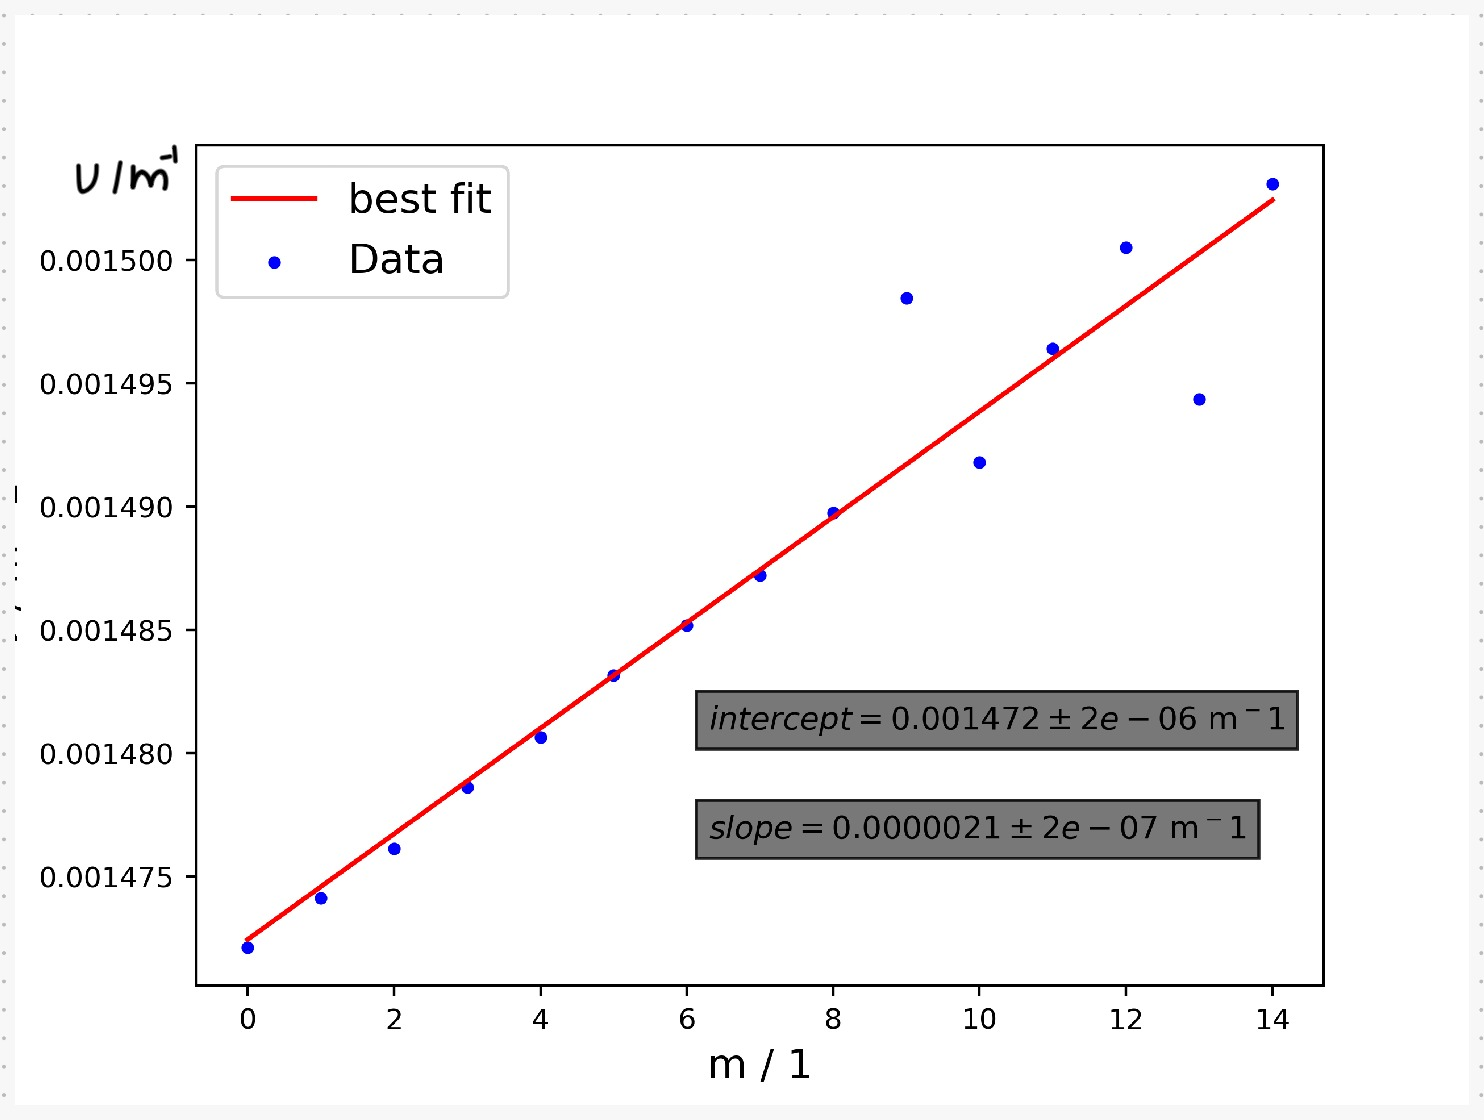
\includegraphics[width=\textwidth]{reg}
		\captionof{figure}{gefittete Gerade, um die Steigung $a$ (slope) und die Konstante $\kappa$ (intercept) zu bestimmen}
		\label{fig:steigung}
	\end{minipage}
\end{center}

\newpage

\noindent Da $n_P$ aus der Tabelle in der Aufgabenstellung entnommen werden kann, kann anhand der Steigung $a$ der gefitteten Geraden die Dicke $d$ der Glasplatte nach \autoref{eq:dicke} bestimmt werden. Der verwendete Wert für die Brechzahl ist dabei 1,520.

%Wert
\begin{equation}
	d = \frac{1}{2n_P a}
	\label{eq:dicke}
\end{equation}

\noindent Daraus ergibt sich für die Dicke $d$ der Platte folgender Wert:

\begin{align*}
	d = \SI{160(20)}{\mu \meter}
\end{align*}

\section{Diskussion}\label{disk}

\subsection{Transmission und Extinktion}

\noindent Die erhaltenen Transmissions- und Extinktionsgraphen stimmen in Etwa mit dem erwarteten Verlauf überein. Betrachtet man die Fehlerbalken, so fällt auf, dass diese, vor allem im kurzwelligen Bereich sehr groß sind. Der direkte Vergleich in \autoref{fig:geg} von beiden Filtern und der Addition der einzelnen Filter, zeigt auch, dass die Graphen sich vor allem im kurzwelligen Bereich deutlich voneinander unterscheiden, während sie ab einer Wellenlänge von 600 nm beinahe deckungsgleich verlaufen, wie es die Theorie für die Additivität der Extinktion voraussagen würde.

\vspace{2mm}

\noindent Der aufgezeichnete Fehler im kurzwelligen Bereich ist vor allem darauf zurückzuführen, dass Spektroskop bei höheren Frequenzen verrauschter aufzeichnet.

\subsection{Stoffmengenkonzentration der Methylenblaulösung}

\noindent Da die genaue Konzentration der Methylenblaulösung nicht bekannt ist, kann keine qualitative Aussage über das erhaltene Ergebnis getätigt werden. Der direkte Vergleich mit den anderen Gruppen zeigt, dass unsere Konzentration deutlich geringer ist. Dies würde sich jedoch auch mit der subjektiven Einschätzung anhand der Blaufärbung der Flüssigkeit decken.

\subsection{Dicke der Glasplatte}

\noindent Auch für die Dicke der Glasplatte ist kein Literaturwert vorhanden, jedoch ist der errechnete Wert in einer realistischen Größenordnung. Der erhaltene Wert wurde auch vor Ort durch Vergleiche mit den anderen Gruppen und Rücksprache mit dem Betreuer verifiziert.

\subsection{Verbesserungsvorschläge}

\noindent Ein Verbesserungsvorschlag wäre, den Versuch in einer geschützten
Umgebung aufzubauen. Dadurch könnten eventuelle Änderungen der
Hintergrundbeleuchtung vermieden werden. Auch können leichte Erschütterungen
des Bodens bereits Fehler verursachen.

\noindent Weiters wären eine bessere Lichtquelle, die garantiert ein konstantes
Lichtspektrum abstrahlen würde, sowie eine bessere Kalibrierung des
Spektrometers durchaus vorteilhaft für ein Besseres Ergebnis, weil der davon
verursachte Fehler, aufgrund der statistischen Auswertung des Versuchs
vernachlässigt wurde.

\noindent Ein weiterer Verbesserungsvorschlag wäre, die Messung öfter zu
wiederholen, um den Fehler, verursacht durch  einmalige Störfaktoren, besser
ausgleichen zu können.

\noindent Das Ergebnis könnte auch verbessert werden, indem man die Filter und
Küvetten gründlich reinigt, sodass keine Streuung durch Verunreinigungen der
Oberfläche zustande kommen kann.

\section{Zusammenfassung}

\noindent Anhand des Versuchs konnte die Additivität der Extinktion leider nur für große Wellenlängen verifiziert werden. Bei den Kurzen Wellenlängen konnte eine Abweichung zum theoretischen Verlauf festgestellt werden, was, wie bereits unter Diskussion erwähnt, verschiedenen Ursachen haben könnte.

\vspace{2mm}

\noindent Die Messungen der Konzentration $c$ der Methylenblaulösung leifert folgendes Ergebnis.

\begin{align*}
	c =  \SI{3.1(2)e-8}{\mol\per\liter}
	%(3,1 \pm 0,2) \,10^{-8} \frac{mol}{l}
\end{align*}

\noindent Bei der Bestimmung der Dicke $d$ der Glasplatte liegt das erhaltene Ergebnis in
der richtigen Größenordnung und ist im folgenden nochmals aufgelistet.

\begin{align*}
	d = \SI{160(20)}{\mu \meter}
	%(160 \pm 20) \mu m
\end{align*}

\newpage

\printbibliography
\listoffigures
\listoftables
\end{document}



%Vorlagen
%

%Gleichungen werden so oder mit \begin{equation} formatiert

%Zitate
%\cite{erstes Wort}


%Unterdrücken von Einrücken
%\noindent 

%referenzen
% \aotoref{name}

%für Formeln $ f $
%\subsection{Idealisierungen}

%Gleichung

%\begin{equation}
%	k_{pos} = \frac{4}{300} \frac{V}{\mu\mathrm{s}} = 13333 \, \frac{V}{s}
%\end{equation}

%\begin{align}
%	 \ddot \phi -\frac{g}{l} \cdot \phi &=0 \label{eq:harm}\\
%     \frac{\text{d}^{2}}{\text{dt}^{2}} [\sin(\omega t)]  - \frac{g}{l} \cdot \sin(\omega t) &= 0 \\ 
%     \therefore \quad \omega^{2}&=\frac{g}{l} \label{eq:omega}
%\end{align}


%\begin{align}
%    T &= 2\pi \sqrt{\frac{l}{g}} \label{eq:reg_sqrt} \\
%    T^{2} &= \frac{4\pi^{2}}{g} l \label{eq:reg_lin} 
%\end{align}

%Kompliziertes Bild

%\begin{minipage}{\textwidth}
%\begin{minipage}[t]{0.43\textwidth}
%	\includegraphics[width=\textwidth]{pics/toplot.PNG}
%\end{minipage}
%\begin{minipage}[t]{0.45\textwidth}
%	\includegraphics[width=\textwidth]{pics/bottomlot.PNG}
%\end{minipage}
%	\captionof{figure}{Ansicht von Oben (Rechts) und von Unten (Links) des Senklots}
%	\label{fig:Senklot}
%    \vspace{1em}
%\end{minipage}



%\begin{minipage}{\textwidth}
%\begin{minipage}[t]{0.59\textwidth}
%    \centering
%    \includegraphics[width=\textwidth]{pics/Aufhangung.jpeg}
%    \captionbelowof{figure}{Aufhängung}
%    \label{fig:Aufhaengung}
%\end{minipage}
%\begin{minipage}[t]{0.40\textwidth}
%    \centering
%    \includegraphics[width=\textwidth]{pics/PendelAufbau.png}
%    \captionof{figure}{Versuchsaufbau}
%    \label{fig:Aufbau}
%\end{minipage}
%    \vspace{1em}
%\end{minipage}

%\begin{wrapfigure}[]{r}{0.4\textwidth}
%\begin{tabular}{@{}l@{}}
%\begin{minipage}{\textwidth}
%\includegraphics[width=0.38\textwidth]{pics/Aufhangung.jpeg}
%\noindent \captionbelowof{figure}{Aufhängung}
%\label{fig:Aufhaengung}
%\end{minipage}\\
%\begin{minipage}{\textwidth}
%\includegraphics[width=0.38\textwidth]{pics/PendelAufbau.png}
%\captionof{figure}{Versuchsaufbau}
%\label{fig:Aufbau}
%\end{minipage}
%\end{tabular}
%\end{wrapfigure}


%Tabelle

%\begin{align}
%	\Delta \bar T_{10} &= t \sigma_{\bar T_{10}} + \Delta T_{res} = \frac{t}{\sqrt{N}}\sigma_{T_{10}}+\Delta T_{res}\\
%	\Delta \bar T &= \frac{ \Delta \bar T_{10}}{10}
%\end{align}


%Tabelle
%
%\begin{table}[htbp]
%\centering
%\begin{tabular}{c|c|c|c|l}
%    [$\frac{\text{m}}{\text{s}^{2}}$] & Literaturwert & Wurzel Fit & Linearer Fit &\\ \hline
%    $g$ & \num{9.806191} & \num{9.79} & \num{9.80} &\\
%    $\Delta g$ & \num{1.2e-5} & \num{1e-2}& \num{1e-2} &\\
%\end{tabular}
%	\captionbelowof{table}{Vergleich mit Literaturwert}
%	\label{Tab:Vergleich}
%\end{table}


%\begin{align}
%	& \Delta T_{\phi} = 2\pi \sqrt{ \frac{l}{g} } \frac{\phi^{2}}{16} = 0.0052\,\text{s} 
%\end{align}
